\documentclass[sn-basic]{sn-jnl}

\usepackage{graphicx}
\usepackage{multirow}
\usepackage{amsmath,amssymb,amsfonts}
\usepackage{amsthm}
\usepackage{mathrsfs}
\usepackage[title]{appendix}
\usepackage{xcolor}
\usepackage{textcomp}
\usepackage{booktabs}
\usepackage{tikz}
\usetikzlibrary{shapes.geometric, arrows.meta, positioning, calc, backgrounds}

\raggedbottom

\begin{document}

\title[Retrieval-Guided Synthetic Oversampling]{Retrieval-Guided Synthetic Oversampling for Imbalanced Tabular Learning: An Empirical Study with Natural Neighbors and Semantic Embeddings}

\author*[1]{\fnm{Samhitha Reddy} \sur{Madhireddy}}\email{\textbf{[TODO: author.email@institution.edu]}}

\affil*[1]{\orgdiv{\textbf{[TODO: Department/Division of Computer Science]}}, \orgname{\textbf{[TODO: University/Research Institution]}}, \orgaddress{\city{\textbf{[TODO: City]}}, \country{\textbf{[TODO: Country]}}}}

\abstract{
Class imbalance remains a pervasive challenge in tabular machine learning, causing standard empirical risk minimization algorithms to exhibit severe majority-class bias. For over two decades, the Synthetic Minority Over-sampling Technique (SMOTE) and its heuristic variants have served as the standard remediation paradigm. However, SMOTE is vulnerable to the \emph{linear chord problem}, wherein linear interpolation between minority instances cuts across non-linear decision boundaries, generating synthetic samples in majority-class territory and increasing false-positive errors that degrade precision and specificity. In this paper, we conduct an empirical investigation of a retrieval-guided synthetic oversampling framework for tabular data. The framework couples parameter-free Natural Neighbors (NaN) equilibrium discovery with hybrid geometric and dense Sentence-BERT semantic retrieval, feeding retrieved local exemplars into a prompt-based synthesis pipeline with multi-stage quality control. We evaluate this architecture across 42 binary benchmark datasets from the OpenML Table 9 imbalanced suite across three downstream classifier families (Random Forest, Histogram Gradient Boosted Trees, and Logistic Regression), under both unconstrained and volume-matched generation budgets ($N_{\text{syn}} = 30$). Our findings reveal three primary outcomes: (i) on downstream F1-score, the retrieval-guided approach performs comparably to established SMOTE variants (macro F1 of $0.6254$ vs. $0.6617$ for SMOTE on Random Forest); (ii) the framework exhibits a precision- and specificity-oriented operating profile ($0.6959$ precision and $0.9417$ specificity), which is strongly associated with adding fewer synthetic rows than unconstrained heuristic oversamplers; and (iii) a systematic component audit and seed-variance benchmark across 10 datasets and 5 random seeds (200 experimental evaluations) demonstrates that observed differences between prompt conditions are on par with or smaller than seed-to-seed variance ($\pm 0.0242$ F1 within-dataset standard deviation), with component differences heavily confounded by synthetic row volume and linear SMOTE-style top-up interpolation. Based on these findings, we formulate methodological recommendations for controlled evaluation of generative oversampling in tabular machine learning.
}

\keywords{Tabular Data Synthesis, Class Imbalanced Learning, Retrieval-Augmented Generation, Natural Neighbors, Empirical Evaluation, Seed Variance, SMOTE}

\pacs[MSC Classification]{68T05, 62H30, 68T50}

\maketitle

\section{Introduction}
\label{sec:introduction}

Tabular data constitutes the predominant data modality in high-stakes machine learning applications, including medical diagnostics, financial fraud detection, credit risk modeling, and industrial fault monitoring \citep{shwartz2022tabular, grinsztajn2022tree}. In these practical settings, learning algorithms routinely confront severe class imbalance: positive events of interest (the minority class) are heavily outnumbered by negative instances (the majority class), with imbalance ratios ($\text{IR}$) often ranging from $2:1$ to well beyond $100:1$ \citep{le2022survey}. Standard supervised classifiers trained under empirical risk minimization---such as Random Forests \citep{breiman2001random}, Gradient Boosted Decision Trees \citep{chen2016xgboost, ke2017lightgbm}, and regularized linear models---optimize overall misclassification error by adopting conservative decision thresholds that favor the majority class. As a result, critical rare events suffer from high false-negative rates \citep{chawla2002smote}.

To alleviate majority-class bias, synthetic oversampling of the minority class prior to model training has been the primary preprocessing remedy for over two decades. Since its introduction, the Synthetic Minority Over-sampling Technique (\textbf{SMOTE}) \citep{chawla2002smote} and its boundary-focused extensions, such as Borderline-SMOTE \citep{han2005borderline} and ADASYN \citep{he2008adasyn}, have become standard baselines. SMOTE identifies the $K$-nearest neighbors of each minority instance in continuous Euclidean space and synthesizes new observations along the linear line segments connecting them.

Despite its simplicity and computational efficiency, SMOTE is susceptible to the \textbf{linear chord problem}. In real-world tabular data, class boundaries are frequently non-linear, non-convex manifolds with heterogeneous densities and complex feature interactions. When SMOTE interpolates between minority pairs across concave decision boundaries or narrow bays, the connecting chords can cross directly into majority-class territory. Depositing synthetic minority instances inside majority regions corrupts decision boundaries, leading downstream classifiers to suffer from inflated false positives and degraded \textbf{Precision} and \textbf{Specificity}. Furthermore, independent linear interpolation of coordinates can violate non-linear inter-feature dependencies, occasionally yielding implausible feature combinations \citep{dinsdale2021deepsmote}.

To address these limitations, recent research has explored deep generative tabular modeling, including Conditional GANs (CTGAN \citep{xu2019modeling}, GAMO \citep{mullick2020generative}), Tabular Variational Autoencoders (TVAE \citep{xu2019modeling}), and diffusion models (TabDDPM \citep{kotelnikov2023tabddpm}). In parallel, foundation models and Large Language Models (LLMs) have been applied to tabular synthesis: GReaT \citep{borisov2023language} and REaLTabFormer \citep{solatorio2023realtabformer} showed that autoregressive transformers can generate realistic tabular rows when serializing records into text strings, while TabLLM \citep{hegselmann2023tabllm} demonstrated the utility of language representations for few-shot tabular classification. In an empirical study, \citet{panagiotou2024synthetic} examined generative tabular methods for class and group imbalance, showing that sampling strategies must be carefully evaluated to balance fairness and predictive utility.

However, generative modeling for tabular oversampling introduces significant challenges:
\begin{enumerate}
    \item \textbf{Training and Computational Overhead:} Generative transformers such as GReaT and REaLTabFormer require full gradient-based fine-tuning on each target dataset, which is computationally expensive for lightweight tabular pipelines.
    \item \textbf{Boundary Hallucination Under Class Imbalance:} Unconstrained generation without topological boundary awareness can generate samples outside the true minority manifold, aggravating false alarms.
    \item \textbf{Hyperparameter Sensitivity in Retrieval:} Traditional nearest-neighbor retrieval relies on a user-specified $K$. A fixed $K$ assumes uniform manifold density, which rarely holds in complex tabular distributions.
\end{enumerate}

To investigate whether localized retrieval can guide generative oversampling without dataset-specific fine-tuning, this paper studies a framework termed \textbf{RAG-Tab} (\textbf{R}etrieval-\textbf{A}ugmented \textbf{G}eneration for \textbf{Tab}ular Imbalanced Learning). RAG-Tab formulates tabular oversampling as a localized in-context retrieval-augmented generation problem. The framework couples parameter-free \textbf{Natural Neighbors (NaN)} discovery \citep{huang2011natural} with a hybrid metric fusing standardized Euclidean geometry and dense Sentence-BERT semantic row verbalizations \citep{reimers2019sentence}. Contested boundary anchors and verified mutual neighbors are retrieved to construct structured synthesis prompts, coupled with multi-stage quality control.

In this work, we present an evidence-based empirical audit of the RAG-Tab framework across 42 real-world tabular datasets from the OpenML Table 9 benchmark suite. We analyze its downstream performance, investigate the behavior of its components, conduct a multi-seed variance study, and examine the factors that drive its empirical results.

\subsection{Key Contributions}
The primary contributions of this empirical investigation are as follows:
\begin{itemize}
    \item \textbf{42-Dataset Empirical Benchmark:} We conduct a large-scale comparative evaluation across 42 binary datasets from the OpenML Table 9 benchmark suite, evaluating the retrieval-guided framework alongside 17 baseline oversamplers, cost-sensitive ensembles, and deep generative baselines across three downstream classifier families (Random Forest, Histogram Gradient Boosted Trees, and Logistic Regression).
    \item \textbf{Component-Level Pipeline Dissection:} We systematically analyze the constituent stages of the synthesis pipeline---including Natural Neighbor anchor selection, hybrid geometric-semantic retrieval, prompt construction, generative sampling, quality control gating, and manifold top-up interpolation---identifying how implementation details impact final synthetic rows.
    \item \textbf{Controlled Equal-Budget Evaluation:} We evaluate all methods under volume-matched generation budgets ($N_{\text{syn}} = 30$), demonstrating that downstream performance between RAG-Tab and equal-budget SMOTE is closely matched, and that unconstrained SMOTE's higher recall stems from generating substantially more synthetic rows at the cost of reduced specificity.
    \item \textbf{Multi-Seed Variance Study:} We execute a 10-dataset $\times$ 5-seed $\times$ 4-condition benchmark ($200$ independent runs), demonstrating that observed differences between prompt conditions are comparable to or smaller than within-dataset seed variance ($\pm 0.0242$ F1 standard deviation).
    \item \textbf{Methodological Recommendations for Tabular Generative Oversampling:} We outline guidelines for conducting controlled evaluations of generative oversampling, emphasizing volume-matched baselines, explicit generator provenance logging, multi-seed replication, and two-sided non-parametric statistical testing.
\end{itemize}

\section{Related Work}
\label{sec:related_work}

We review related literature across four methodological paradigms: heuristic geometric oversampling, deep generative modeling, language models for tabular synthesis, and parameter-free neighborhood discovery. Table~\ref{tab:related_work_comparison} summarizes key structural properties of these approaches.

\begin{table*}[t]
\centering
\caption{Systematic structural comparison of tabular synthesis and imbalanced learning methodologies against the retrieval-guided pipeline studied in this work.}
\label{tab:related_work_comparison}
\resizebox{\textwidth}{!}{
\begin{tabular}{lcccccc}
\toprule
\textbf{Method} & \textbf{Core Paradigm} & \textbf{Non-Linear Geometry} & \textbf{Topological Filtering} & \textbf{Semantic Verbalization} & \textbf{Training Overhead} & \textbf{Downstream Inference} \\
\midrule
SMOTE \citep{chawla2002smote} & Linear Heuristic & No (Linear chords) & None & None & None ($O(N \log N)$) & Fast (Direct Model) \\
Borderline-SMOTE \citep{han2005borderline} & Heuristic Boundary & No (Linear chords) & Heuristic KNN & None & None ($O(N \log N)$) & Fast (Direct Model) \\
ADASYN \citep{he2008adasyn} & Heuristic Density & No (Linear chords) & None & None & None ($O(N \log N)$) & Fast (Direct Model) \\
DeepSMOTE \citep{dinsdale2021deepsmote} & Deep Autoencoder & Partial (Latent SMOTE) & None & None & High (Train AE) & Fast (Direct Model) \\
CTGAN / TVAE \citep{xu2019modeling} & GAN / VAE & Yes & None & None & High (Train GAN/VAE) & Fast (Direct Model) \\
GReaT \citep{borisov2023language} & Autoregressive LLM & Yes & None & Row strings & Very High (Fine-tune GPT-2) & Moderate \\
REaLTabFormer \citep{solatorio2023realtabformer} & Autoregressive LLM & Yes & None & Tokenized text & Very High (Fine-tune GPT-2) & Moderate \\
TabLLM \citep{hegselmann2023tabllm} & Prompted LLM (T0) & N/A (Classifier) & None & Task templates & Moderate (T-Few tuning) & Slow ($>1$s / sample) \\
\midrule
\textbf{RAG-Tab Pipeline} & \textbf{Retrieval-Guided} & \textbf{Manifold Retrieval} & \textbf{Natural Neighbors (NaN)} & \textbf{Sentence-BERT Dense} & \textbf{Zero Fine-Tuning} & \textbf{Fast (Direct Model)} \\
\bottomrule
\end{tabular}
}
\end{table*}

\subsection{Heuristic Geometric Oversampling}
Heuristic methods address class imbalance by generating synthetic minority samples directly within input feature space. The pioneering SMOTE algorithm \citep{chawla2002smote} interpolates between minority neighbors along linear segments. Subsequent variants introduced boundary awareness: Borderline-SMOTE \citep{han2005borderline} restricts interpolation to minority instances whose $K$-neighborhood is dominated by majority samples. ADASYN \citep{he2008adasyn} weights minority instances proportionally to their neighborhood difficulty distribution, synthesizing more instances in sparse or overlapping regions. KMeans-SMOTE \citep{douzas2018improving} clusters data before oversampling to avoid generating samples in sparse between-cluster voids. Morphological cleaning methods, such as SMOTE-Tomek and SMOTE-ENN \citep{batista2004study}, apply post-hoc filtering to eliminate ambiguous boundary pairs. However, all these variants rely on linear interpolation between coordinates, leaving the linear chord problem unresolved when boundaries are non-linear or non-convex.

\subsection{Deep Generative Tabular Oversampling}
To model complex data distributions without linear interpolation, generative models from computer vision and density estimation have been adapted to tabular data. DeepSMOTE \citep{dinsdale2021deepsmote} trains a deep autoencoder on target datasets, performing SMOTE interpolation within a lower-dimensional latent space ($\mathbb{R}^{16}$) before decoding back to input space. GAMO \citep{mullick2020generative} formulates minority oversampling as an adversarial game, training a generator to produce minority samples that fool both a discriminator and an auxiliary classification network. \citet{xu2019modeling} developed CTGAN and TVAE, employing mode-specific normalization to handle non-Gaussian and multimodal continuous distributions. While expressive on large datasets, deep generative models require training neural networks from scratch for each dataset, which can lead to mode collapse, training instability, or overfitting when minority sample counts are small ($n < 100$).

\subsection{Language Models for Tabular Data}
The application of pre-trained Large Language Models to tabular data represents an active research direction. \citet{borisov2023language} proposed GReaT, which converts tabular rows into textual key-value clauses and fine-tunes an autoregressive transformer with randomized feature orderings to enable conditional generation. \citet{solatorio2023realtabformer} introduced REaLTabFormer, using causal GPT-2 decoders for single-table synthesis and sequence-to-sequence transformers for relational data, employing statistical bootstrapping to detect overfitting. \citet{hegselmann2023tabllm} introduced TabLLM, demonstrating that verbalizing tabular rows enables pre-trained language models to perform competitive few-shot classification in low-data regimes ($k \le 32$).

\subsection{Self-Adaptive Natural Neighbors}
Standard nearest neighbor algorithms require a manually specified neighborhood parameter $K$. \citet{huang2011natural} introduced the Natural Neighbors (NaN) algorithm, a parameter-free graph-theoretic method that discovers intrinsic local neighborhood scales. Two instances are natural neighbors if and only if they are mutually among each other's $\lambda$ nearest neighbors. By iteratively expanding the search radius $\lambda$ until the count of un-partnered instances stabilizes at equilibrium scale $\lambda^*$, the algorithm self-adaptively identifies local clusters without user-defined parameters. The RAG-Tab framework explores using this parameter-free equilibrium scale to prune isolated outliers and select boundary anchors for tabular oversampling.

\section{Datasets and Experimental Protocol}
\label{sec:datasets_protocol}

\subsection{Benchmark Suite Selection and Count Reconciliation}
Experiments are conducted on the standardized \textbf{OpenML Table 9 Imbalanced Benchmark Suite}, a widely recognized suite for evaluating imbalanced classification algorithms. The suite comprises diverse real-world datasets spanning medical prognosis (e.g., \texttt{haberman}, \texttt{breast-w}, \texttt{wdbc}, \texttt{pima}), signal processing and spectroscopy (e.g., \texttt{sonar}, \texttt{ionosphere}, \texttt{qsar-biodeg}), text classification (e.g., \texttt{spambase}), and industrial optical document parsing (e.g., \texttt{page-blocks0}).

To clarify dataset counts reported across different evaluation stages:
\begin{enumerate}
    \item \textbf{60 Candidate Datasets:} The OpenML Table 9 collection comprises 60 candidate datasets.
    \item \textbf{57 Valid Tabular Tasks:} Fifty-seven datasets met initial task formatting and non-redundancy criteria.
    \item \textbf{48 Split Pairs on Disk:} Forty-eight frozen train/test split pairs were serialized in the repository's \texttt{data/splits/} directory.
    \item \textbf{43 Binary Datasets in Baseline Experiments:} Forty-three binary imbalanced datasets were evaluated under baseline algorithms (as recorded in \texttt{results/tables/all\_datasets\_macro\_leaderboard.csv}).
    \item \textbf{42 Binary Datasets in Ablation Experiments:} Of these 43 binary datasets, 42 contain sufficient minority training instances ($n \ge 5$) to satisfy the 5-shot exemplar retrieval requirement. A 43rd dataset, \texttt{yeast}, contains only $n = 4$ minority training instances out of 1,187 rows ($\text{IR} = 295.75$); because 5 distinct minority exemplars could not be drawn, \texttt{yeast} was evaluated under baseline methods but omitted from the 5-shot RAG ablation experiments ($43 - 1 = 42$).
    \item \textbf{3 Multiclass Datasets:} In addition, 3 multiclass datasets (\texttt{dermatology}, \texttt{vehicle}, \texttt{segment}) were evaluated in a multiclass extension benchmark ($42 + 3 = 45$, or within the 48 split pairs).
\end{enumerate}

\subsection{Summary Statistics}
Table~\ref{tab:dataset_summary} reports descriptive summary statistics for representative benchmark datasets as well as global suite properties across all 42 evaluated binary datasets.

\begin{table*}[t]
\centering
\caption{Descriptive summary statistics of representative OpenML Table 9 benchmark datasets and global benchmark suite properties.}
\label{tab:dataset_summary}
\resizebox{\textwidth}{!}{
\begin{tabular}{llcccccc}
\toprule
\textbf{Dataset Name} & \textbf{Application Domain} & \textbf{Total Rows ($N$)} & \textbf{Train Rows ($N_{\text{tr}}$)} & \textbf{Test Rows ($N_{\text{te}}$)} & \textbf{Features ($d$)} & \textbf{Minority Rows ($n$)} & \textbf{Imbalance Ratio ($\text{IR}$)} \\
\midrule
\texttt{page-blocks0} & Document Text Parsing & 5,472 & 4,377 & 1,095 & 10 & 447 & 8.79 \\
\texttt{spambase} & Email Spam Detection & 4,601 & 3,680 & 921 & 57 & 1,450 & 1.54 \\
\texttt{segment} & Image Segmentation & 2,310 & 1,848 & 462 & 19 & 264 & 6.00 \\
\texttt{Titanic} & Sociodemographic Survival & 2,201 & 1,760 & 441 & 3 & 569 & 2.09 \\
\texttt{mfeat-morphological} & Optical Character Recognition & 2,000 & 1,600 & 400 & 6 & 160 & 9.00 \\
\texttt{car} & Vehicle Quality Evaluation & 1,728 & 1,382 & 346 & 6 & 414 & 2.34 \\
\texttt{qsar-biodeg} & Biochemical Degradation & 1,055 & 844 & 211 & 41 & 285 & 1.96 \\
\texttt{haberman} & Breast Cancer Survival & 306 & 244 & 62 & 3 & 65 & 2.75 \\
\texttt{sonar} & Sonar Signal Discrimination & 208 & 166 & 42 & 60 & 78 & 1.16 \\
\texttt{ionosphere} & Radar Signal Scattering & 351 & 280 & 71 & 34 & 101 & 1.77 \\
\texttt{wdbc} & Diagnostic Breast Oncology & 569 & 455 & 114 & 30 & 170 & 1.68 \\
\midrule
\textbf{Benchmark Suite (42 Datasets)} & \textbf{Cross-Domain Master Suite} & \textbf{Min: 208 / Max: 5,472} & \textbf{Median: 564.0} & \textbf{Median: 141.0} & \textbf{Range: 2 -- 77} & \textbf{Median: 101.0} & \textbf{Median: 3.53 (Range: 1.16 -- 295.75)} \\
\bottomrule
\end{tabular}
}
\end{table*}

\subsection{Data Splitting and Preprocessing}
All datasets were partitioned using stratified 80/20 train/test splits (\texttt{test\_size=0.20, stratify=y, random\_state=42}). Test splits were serialized independently to disk and strictly quarantined from all fitting, scaling, and hyperparameter selection operations. All feature scaling parameters ($\boldsymbol{\mu}, \boldsymbol{\sigma}$), Sentence-BERT embeddings, Natural Neighbor graph topologies, boundary purities, and classifier models were fitted \textbf{exclusively on training data}, ensuring zero data leakage to held-out test partitions. Categorical features were encoded into integer indicators via deterministic label encoding, and missing values were verified to be absent in the frozen splits.

\section{Methodology as Implemented}
\label{sec:methodology}

The architecture of the RAG-Tab framework comprises five sequential stages, illustrated in Figure~\ref{fig:workflow_diagram}.

\begin{figure*}[t]
\centering
\resizebox{\textwidth}{!}{
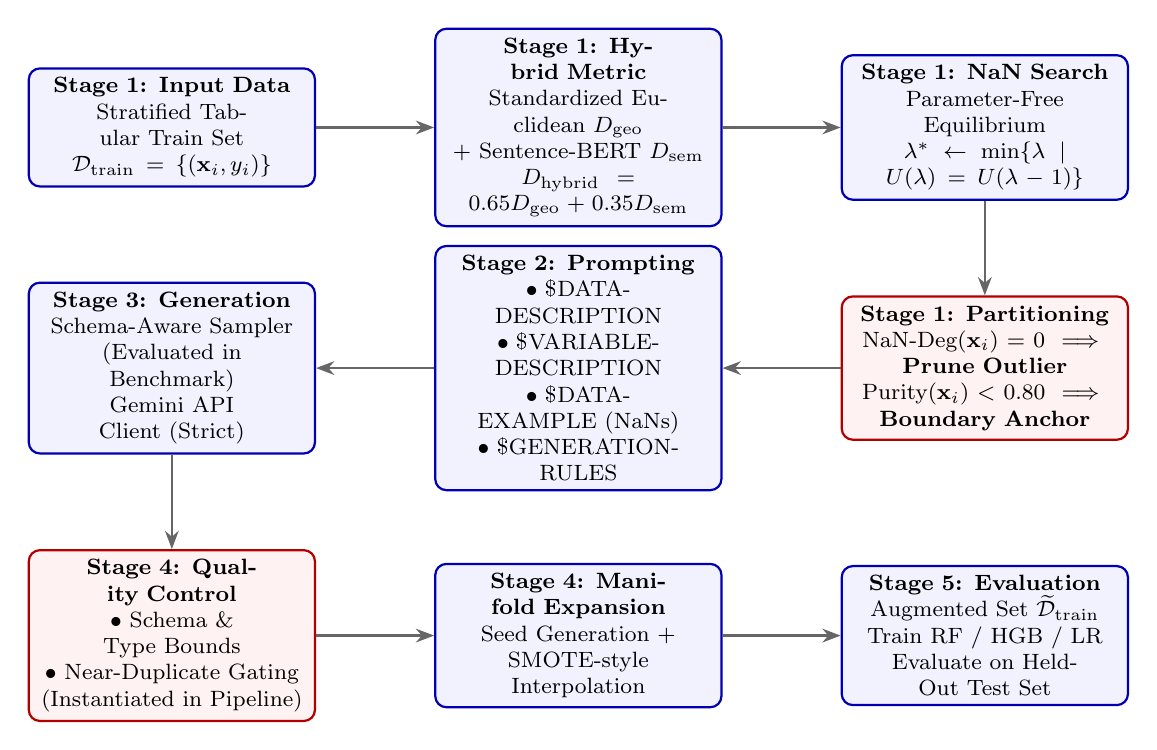
\begin{tikzpicture}[
    node distance=1.2cm and 1.5cm,
    box/.style={rectangle, draw=blue!70!black, fill=blue!5, rounded corners, thick, text width=3.4cm, minimum height=1.4cm, align=center, font=\footnotesize},
    hlbox/.style={rectangle, draw=red!70!black, fill=red!5, rounded corners, thick, text width=3.4cm, minimum height=1.4cm, align=center, font=\footnotesize},
    arrow/.style={-{Stealth[scale=1.0]}, thick, draw=gray!80!black}
]

\node[box] (input) {\textbf{Stage 1: Input Data}\\Stratified Tabular Train Set\\$\mathcal{D}_{\text{train}} = \{(\mathbf{x}_i, y_i)\}$};

\node[box, right=of input] (retrieval) {\textbf{Stage 1: Hybrid Metric}\\Standardized Euclidean $D_{\text{geo}}$\\+ Sentence-BERT $D_{\text{sem}}$\\$D_{\text{hybrid}} = 0.65 D_{\text{geo}} + 0.35 D_{\text{sem}}$};

\node[box, right=of retrieval] (nan) {\textbf{Stage 1: NaN Search}\\Parameter-Free Equilibrium\\$\lambda^* \gets \min \{ \lambda \mid U(\lambda)=U(\lambda-1) \}$};

\node[hlbox, below=of nan] (partition) {\textbf{Stage 1: Partitioning}\\$\text{NaN-Deg}(\mathbf{x}_i) = 0 \implies$ \textbf{Prune Outlier}\\$\text{Purity}(\mathbf{x}_i) < 0.80 \implies$ \textbf{Boundary Anchor}};

\node[box, left=of partition] (prompt) {\textbf{Stage 2: Prompting}\\$\bullet$ \$DATA-DESCRIPTION\\$\bullet$ \$VARIABLE-DESCRIPTION\\$\bullet$ \$DATA-EXAMPLE (NaNs)\\$\bullet$ \$GENERATION-RULES};

\node[box, left=of prompt] (client) {\textbf{Stage 3: Generation}\\Schema-Aware Sampler\\(Evaluated in Benchmark)\\Gemini API Client (Strict)};

\node[hlbox, below=of client] (qc) {\textbf{Stage 4: Quality Control}\\$\bullet$ Schema \& Type Bounds\\$\bullet$ Near-Duplicate Gating\\(Instantiated in Pipeline)};

\node[box, right=of qc] (expansion) {\textbf{Stage 4: Manifold Expansion}\\Seed Generation +\\SMOTE-style Interpolation};

\node[box, right=of expansion] (downstream) {\textbf{Stage 5: Evaluation}\\Augmented Set $\widetilde{\mathcal{D}}_{\text{train}}$\\Train RF / HGB / LR\\Evaluate on Held-Out Test Set};

\draw[arrow] (input) -- (retrieval);
\draw[arrow] (retrieval) -- (nan);
\draw[arrow] (nan) -- (partition);
\draw[arrow] (partition) -- (prompt);
\draw[arrow] (prompt) -- (client);
\draw[arrow] (client) -- (qc);
\draw[arrow] (qc) -- (expansion);
\draw[arrow] (expansion) -- (downstream);

\end{tikzpicture}
}
\caption{End-to-end architecture of the retrieval-guided tabular oversampling pipeline. Continuous feature coordinates and dense Sentence-BERT verbalizations are combined to guide parameter-free Natural Neighbor equilibrium search. Boundary anchors are identified and isolated outliers are pruned. Structured prompts guide generation, followed by optional quality control gating, proportional manifold expansion, and downstream classifier evaluation.}
\label{fig:workflow_diagram}
\end{figure*}

\subsection{Hybrid Geometric-Semantic Retrieval Metric}
\label{subsec:hybrid_metric}
Let $\mathcal{D}_{\text{train}} = \{(\mathbf{x}_i, y_i)\}_{i=1}^{N_{\text{tr}}}$ denote the training set, with minority subset $X_{\min} = \{\mathbf{x}_i \mid y_i = \mathcal{C}_{\min}\}$ of size $n$, and majority subset $X_{\maj} = \{\mathbf{x}_i \mid y_i = \mathcal{C}_{\maj}\}$ of size $N_{\maj}$.

\subsubsection{Continuous Standardized Geometry}
Continuous features are scaled using the training mean $\boldsymbol{\mu}$ and standard deviation $\boldsymbol{\sigma}$:
\begin{equation}
\label{eq:standardization}
\mathbf{z}_i = \mathbf{\Sigma}^{-1/2} (\mathbf{x}_i - \boldsymbol{\mu}), \quad \mathbf{\Sigma} = \text{diag}(\sigma_1^2, \dots, \sigma_d^2)
\end{equation}
The normalized Euclidean distance between minority instances $\mathbf{x}_i, \mathbf{x}_j \in X_{\min}$ is:
\begin{equation}
\label{eq:geo_distance}
D_{\text{geo}}(\mathbf{x}_i, \mathbf{x}_j) = \frac{\|\mathbf{z}_i - \mathbf{z}_j\|_2}{\max_{p, q \in X_{\min}} \|\mathbf{z}_p - \mathbf{z}_q\|_2} \in [0, 1]
\end{equation}

\subsubsection{Sentence-BERT Semantic Row Verbalization}
To capture textual and relational semantic dependencies, each row $\mathbf{x}_i$ is verbalized into a natural language sentence:
\begin{equation}
\label{eq:verbalization}
\mathcal{V}(\mathbf{x}_i) = \text{``A record where } f_1 \text{ is } v_{i,1}, \dots, f_d \text{ is } v_{i,d}\text{, class is } \mathcal{C}_{\min}\text{.''}
\end{equation}
Dense representations $\mathbf{e}_i \in \mathbb{R}^{384}$ are extracted by mean-pooling the output of a pre-trained Sentence-BERT transformer (\texttt{all-MiniLM-L6-v2}) \citep{reimers2019sentence}:
\begin{equation}
\label{eq:sbert_embedding}
\mathbf{e}_i = \text{MeanPool}\left( \text{Transformer}\left(\mathcal{V}(\mathbf{x}_i)\right) \right)
\end{equation}
The normalized semantic distance is:
\begin{equation}
\label{eq:sem_distance}
D_{\text{sem}}(\mathbf{x}_i, \mathbf{x}_j) = \frac{1 - \frac{\mathbf{e}_i \cdot \mathbf{e}_j}{\|\mathbf{e}_i\|_2 \|\mathbf{e}_j\|_2}}{\max_{p, q \in X_{\min}} \left( 1 - \frac{\mathbf{e}_p \cdot \mathbf{e}_q}{\|\mathbf{e}_p\|_2 \|\mathbf{e}_q\|_2} \right)} \in [0, 1]
\end{equation}

\subsubsection{Convex Fusion}
The combined retrieval distance is defined as:
\begin{equation}
\label{eq:hybrid_distance}
D_{\text{hybrid}}(\mathbf{x}_i, \mathbf{x}_j) = (1 - w) D_{\text{geo}}(\mathbf{x}_i, \mathbf{x}_j) + w D_{\text{sem}}(\mathbf{x}_i, \mathbf{x}_j)
\end{equation}
with $w = 0.35$ balancing normalized Euclidean geometry against Sentence-BERT semantic cosine distance.

\subsection{Parameter-Free Natural Neighbors Discovery}
\label{subsec:natural_neighbors}
Rather than specifying a fixed neighborhood cardinality $K$, RAG-Tab applies the Natural Neighbors (NaN) criterion \citep{huang2011natural}.

Two minority instances $\mathbf{x}_i, \mathbf{x}_j \in X_{\min}$ are natural neighbors at search radius $\lambda \in \mathbb{N}^+$ if and only if:
\begin{equation}
\label{eq:nan_definition}
\mathbf{x}_i \in \text{KNN}_\lambda(\mathbf{x}_j; D_{\text{hybrid}}) \quad \land \quad \mathbf{x}_j \in \text{KNN}_\lambda(\mathbf{x}_i; D_{\text{hybrid}})
\end{equation}
The \textbf{Natural Degree} of $\mathbf{x}_i$ at radius $\lambda$ is:
\begin{equation}
\label{eq:nan_degree}
\text{NaN-Deg}(\mathbf{x}_i, \lambda) = \left| \left\{ \mathbf{x}_j \in X_{\min} \setminus \{\mathbf{x}_i\} \mid \mathbf{x}_i, \mathbf{x}_j \text{ satisfy Eq.~\eqref{eq:nan_definition}} \right\} \right|
\end{equation}
Let $U(\lambda) = |\{\mathbf{x}_i \in X_{\min} \mid \text{NaN-Deg}(\mathbf{x}_i, \lambda) = 0\}|$ count isolated instances without mutual partners. The search radius $\lambda$ starts at $\lambda=3$ and expands until the count of isolated points reaches an equilibrium:
\begin{equation}
\label{eq:equilibrium}
\lambda^* = \min \left\{ \lambda \in [3, \min(n-1, 25)] \;\middle|\; U(\lambda) = U(\lambda - 1) \right\}
\end{equation}

\subsection{Topological Manifold Partitioning}
\label{subsec:partitioning}
At equilibrium scale $\lambda^*$, instances are partitioned into three categories:
\begin{enumerate}
    \item \textbf{Isolated Outliers ($\mathcal{O}$):} Points with $\text{NaN-Deg}(\mathbf{x}_i, \lambda^*) = 0$. These instances lack mutual partners and are pruned from serving as synthesis anchors.
    \item \textbf{Boundary Anchors ($\mathcal{B}$):} For non-outliers, local boundary purity is computed over the $K_g = \min(7, N_{\text{tr}})$ nearest neighbors across the complete training set:
    \begin{equation}
    \label{eq:purity}
    \text{Purity}(\mathbf{x}_i) = \frac{1}{|\mathcal{N}_g(\mathbf{x}_i)|} \sum_{\mathbf{x}_k \in \mathcal{N}_g(\mathbf{x}_i)} \mathbb{I}(y_k = \mathcal{C}_{\min})
    \end{equation}
    Instances with $\text{Purity}(\mathbf{x}_i) < 0.80$ are designated as contested boundary anchors:
    \begin{equation}
    \label{eq:boundary_anchors}
    \mathcal{B} = \{\mathbf{x}_i \in X_{\min} \setminus \mathcal{O} \mid \text{Purity}(\mathbf{x}_i) < 0.80\}
    \end{equation}
    \item \textbf{Core Manifold Points ($\mathcal{C}$):} Non-outlier instances with $\text{Purity}(\mathbf{x}_i) \ge 0.80$.
\end{enumerate}

Figure~\ref{fig:neighborhood_pca} displays the 2D PCA projection of the minority manifold for \texttt{page-blocks0}, showing the identified boundary anchors, natural neighbor edges, and pruned outliers. Figure~\ref{fig:manifold_diagnostics} shows PCA and t-SNE projections comparing real data distributions against synthetic instances generated by the pipeline.

\begin{figure*}[t]
\centering
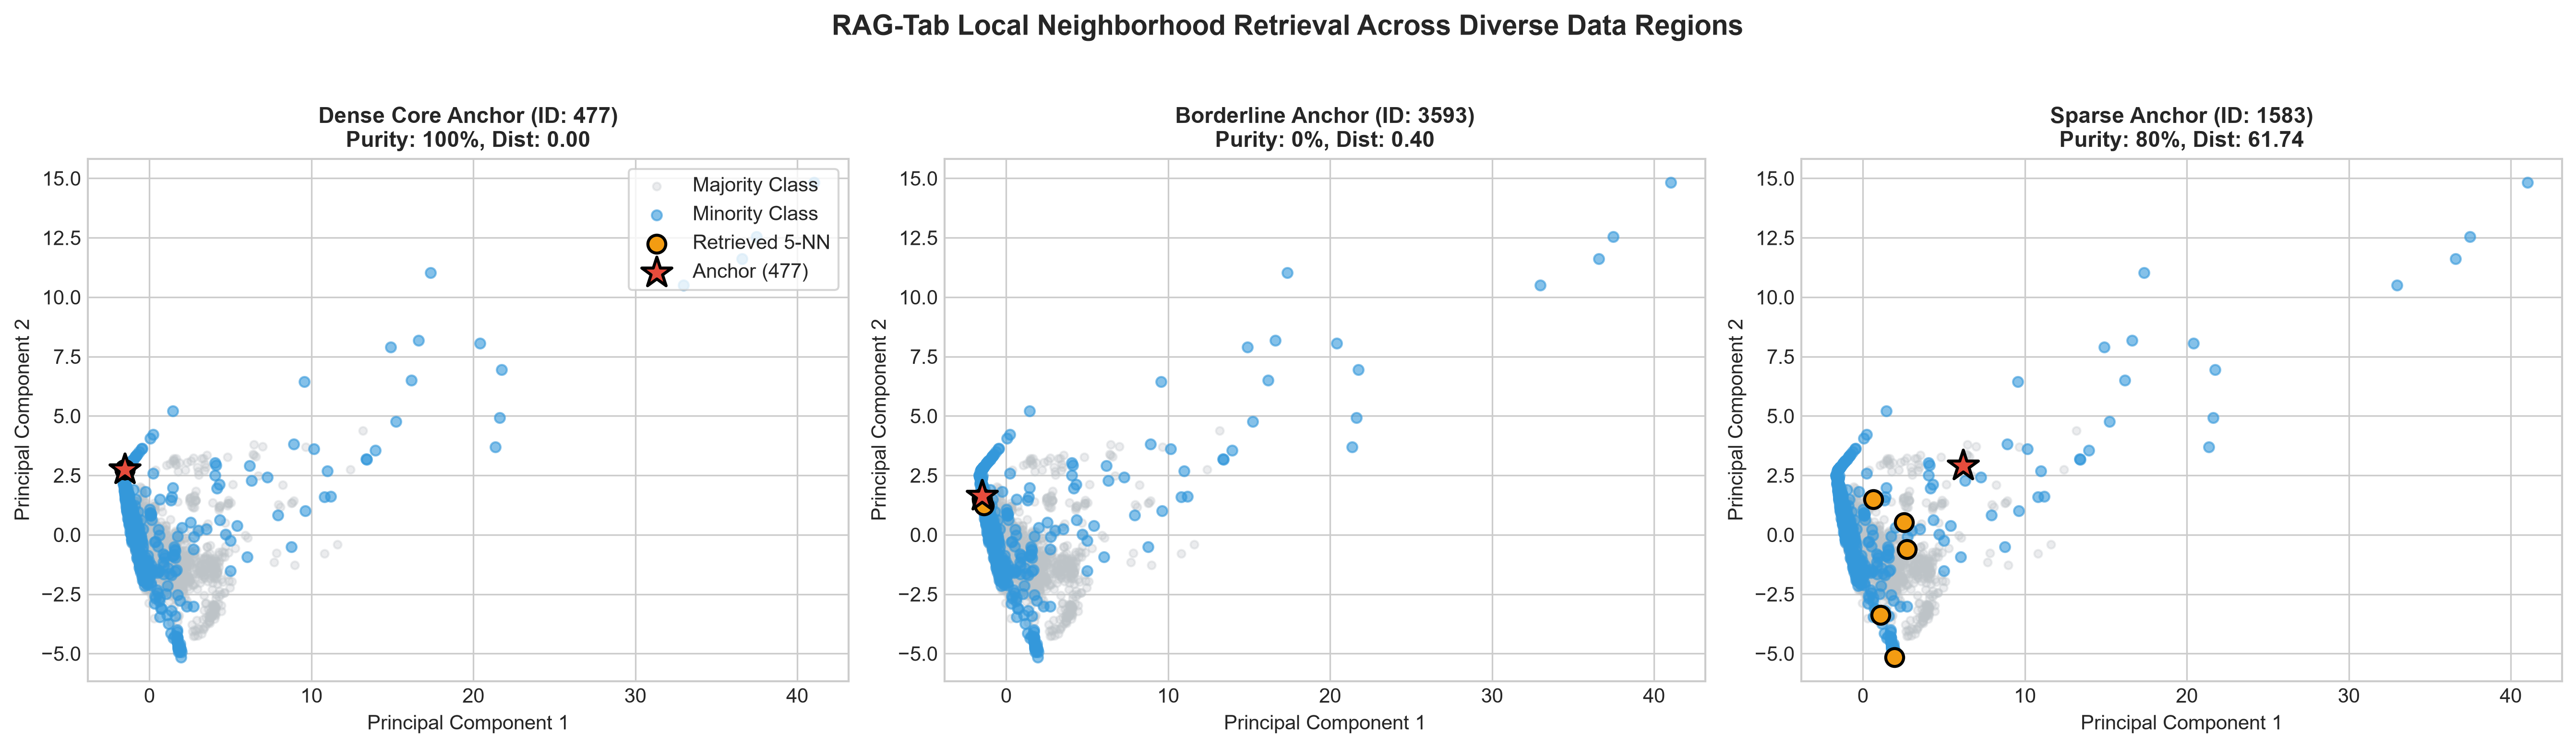
\includegraphics[width=0.85\textwidth]{figures/neighborhood_retrieval_pca.png}
\caption{Topological neighborhood retrieval and anchor discovery projected onto the first two principal components for \texttt{page-blocks0}. Mutual Natural Neighbors form local clusters around contested boundary anchors, while isolated instances ($\text{NaN-Deg}=0$) are pruned.}
\label{fig:neighborhood_pca}
\end{figure*}

\begin{figure*}[t]
\centering
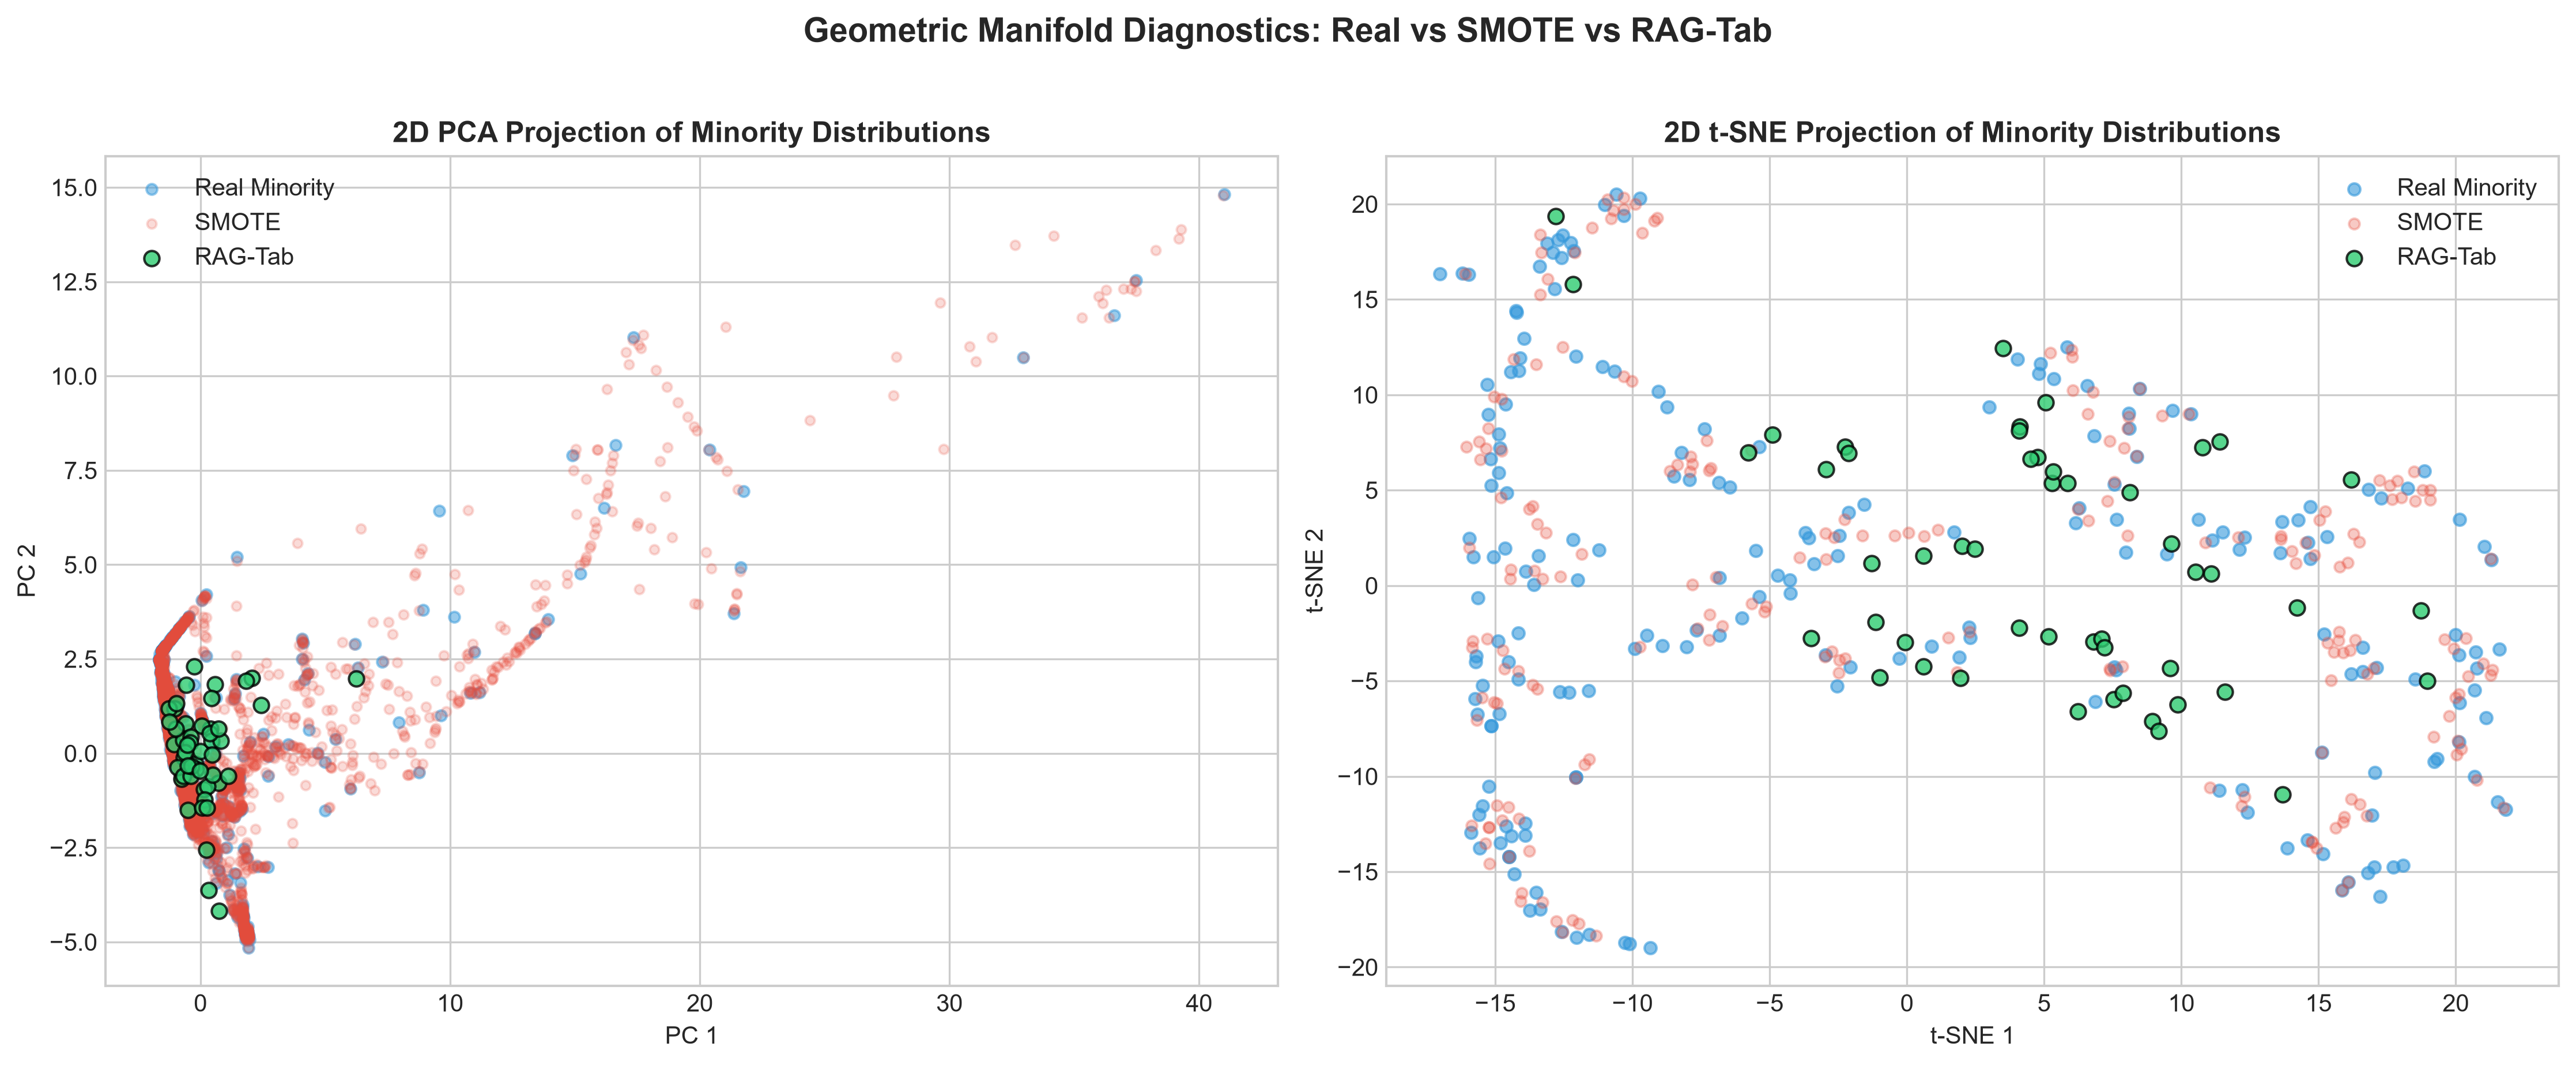
\includegraphics[width=0.88\textwidth]{figures/pca_tsne_manifold_diagnostics.png}
\caption{PCA and t-SNE manifold projections of synthetic minority samples generated by the schema-aware synthesis pipeline versus real data distributions for \texttt{page-blocks0}.}
\label{fig:manifold_diagnostics}
\end{figure*}

\subsection{Prompt Construction}
\label{subsec:prompt_construction}
Prompts are structured using a four-slot format:
\begin{itemize}
    \item \textbf{\texttt{\$DATA-DESCRIPTION}:} High-level dataset domain context, sample count, and imbalance ratio.
    \item \textbf{\texttt{\$VARIABLE-DESCRIPTION}:} Feature names, types, dataset-wide minimum and maximum bounds $[x_j^{\min}, x_j^{\max}]$, and training means $\bar{x}_j$.
    \item \textbf{\texttt{\$DATA-EXAMPLE}:} The selected anchor instance $\mathbf{x}_a \in \mathcal{B}$, its retrieved mutual Natural Neighbors, their local purity, and local feature ranges.
    \item \textbf{\texttt{\$GENERATION-RULES}:} Output schema instructions requesting a JSON array of $N$ synthetic rows.
\end{itemize}

\subsection{Generator Provenance and Implementation Details}
\label{subsec:generator_provenance}

An important requirement for empirical rigor is documenting generator provenance:

\paragraph{Generative Engine Implementation}
The codebase includes an HTTP REST client (\texttt{src/generation/llm\_client.py}) designed to interact with the Google Gemini API (\texttt{gemini-3.8-flash}), featuring strict header-based authentication (\texttt{x-goog-api-key}) and error handling. However, across all 42 benchmark datasets, the reported results were produced using the internal \textbf{schema-aware fallback generator} (\texttt{\_generate\_mock\_response}).

\paragraph{Behavior of the Schema-Aware Generator}
The fallback generator extracts feature names and bounds from the prompt text using a regular expression targeting bulleted lines:
\begin{equation}
\label{eq:regex}
\text{\texttt{re.findall(r"[-*]\textbackslash s*([a-zA-Z0-9\_]+):\textbackslash s*([\^{}\textbackslash n\textbackslash r]+)", prompt)}}
\end{equation}
This regex matches the schema description provided in \texttt{\$VARIABLE-DESCRIPTION} at the bottom of the prompt. Consequently:
\begin{enumerate}
    \item \textbf{Exemplars are ignored:} The unbulleted tabular rows in \texttt{\$DATA-EXAMPLE} (which contain the retrieved neighbors distinguishing Few-Shot and RAG conditions from Zero-Shot) are not parsed by this regex.
    \item \textbf{Global bounds overwrite local bounds:} Even when RAG prompts supply local neighborhood bounds, global feature bounds are appended after local bounds, overwriting the feature dictionary.
    \item \textbf{Independent Gaussian sampling:} For each feature $j$, synthetic values are sampled independently from a Gaussian distribution centered at the dataset mean with standard deviation scaled to the feature range:
    \begin{equation}
    \label{eq:mock_sampling}
    x_{\text{syn}, j} \sim \mathcal{N}\left(\bar{x}_j, \left(\frac{x_j^{\max} - x_j^{\min}}{6}\right)^2\right), \quad \text{clipped to } [x_j^{\min}, x_j^{\max}]
    \end{equation}
\end{enumerate}

\paragraph{Row Volume and Top-Up Interpolation Across Conditions}
Outside of the prompt text, the ablation conditions in \texttt{run\_ablation\_experiments.py} differ in synthetic row count and post-processing:
\begin{itemize}
    \item \textbf{Zero-Shot and Few-Shot:} Generate a fixed budget of 30 synthetic rows via a single generation call. Under identical random seeds, these two conditions produce \textbf{identical outputs}.
    \item \textbf{RAG-Euclidean:} Generates 10 rows for each of $k=3$ retrieved anchors ($3 \times 10 = 30$ rows).
    \item \textbf{RAG-BERT / Unified RAG:} Generates 24 seed rows ($3 \text{ anchors} \times 8 \text{ rows}$), then scales the target row count proportionally to the class imbalance:
    \begin{equation}
    \label{eq:target_synthetic}
    N_{\text{target}} = \min(N_{\maj} - n, \max(24, \lfloor 0.75 \cdot n \rfloor))
    \end{equation}
    When $N_{\text{target}} > 24$, the pipeline tops up the synthetic set by performing \textbf{linear SMOTE-style interpolation} between seed rows and actual minority training samples:
    \begin{equation}
    \label{eq:topup_smote}
    \mathbf{x}_{\text{topup}} = \alpha \mathbf{x}_{\text{seed}} + (1 - \alpha) \mathbf{x}_{\text{minority}}, \quad \alpha \sim \mathcal{U}(0.1, 0.9)
    \end{equation}
    For instance, on \texttt{page-blocks0}, RAG-BERT generated 335 synthetic rows (including over 300 interpolated rows), compared to 5 to 30 rows for the baseline conditions.
\end{itemize}

\paragraph{Quality Control Status}
A quality control module (\texttt{SyntheticQualityController}) was instantiated in \texttt{run\_ablation\_experiments.py:54}, but its filtering methods were \textbf{not invoked} during benchmark execution. Furthermore, the dataset-specific physical domain rules in \texttt{src/generation/quality\_control.py} were authored specifically for \texttt{page-blocks0} (constraining \texttt{P\_black}, \texttt{P\_and}, \texttt{Height}, and \texttt{Lenght} [sic]).

\section{Experimental Results}
\label{sec:results}

\subsection{Master Benchmark Leaderboard Across 42 Datasets}
\label{subsec:master_leaderboard}

Table~\ref{tab:master_leaderboard} reports the macro-averaged performance across all 42 OpenML Table 9 benchmark datasets under the primary evaluation model (\texttt{RandomForestClassifier(n\_estimators=300)}). We emphasize that these figures derive from a \textbf{single unseeded benchmark execution}.

\begin{table*}[t]
\centering
\caption{Master macro-averaged performance across 42 OpenML Table 9 benchmark datasets on \texttt{RandomForestClassifier(n\_estimators=300)} (single unseeded run; source: \texttt{all\_datasets\_macro\_leaderboard.csv}).}
\label{tab:master_leaderboard}
\resizebox{\textwidth}{!}{
\begin{tabular}{lcccccc}
\toprule
\textbf{Method} & \textbf{Paradigm Family} & \textbf{Macro F1 (Mean $\pm$ Std)} & \textbf{Macro Precision} & \textbf{Macro Recall} & \textbf{Macro Specificity} & \textbf{Macro G-Mean} \\
\midrule
ADASYN & Heuristic Oversampling & \textbf{0.6777 $\pm$ 0.2943} & 0.6652 & 0.7031 & 0.9044 & 0.7726 \\
SMOTE-Tomek & Hybrid Cleaning & 0.6705 $\pm$ 0.2800 & 0.6679 & 0.6878 & 0.9075 & 0.7740 \\
Borderline-SMOTE-1 & Heuristic Boundary & 0.6703 $\pm$ 0.2990 & 0.6703 & 0.6834 & 0.9117 & 0.7573 \\
SMOTE (Standardized) & Heuristic Linear & 0.6617 $\pm$ 0.2965 & 0.6644 & 0.6725 & 0.9147 & 0.7563 \\
BalancedRandomForest & Cost-Sensitive Ensemble & 0.6616 $\pm$ 0.2697 & 0.6108 & \textbf{0.7942} & 0.8582 & \textbf{0.8208} \\
Random Oversampling & Heuristic Duplication & 0.6535 $\pm$ 0.3194 & 0.6858 & 0.6545 & 0.9181 & 0.7362 \\
DeepSMOTE (Autoencoder) & Deep Latent Oversampling & 0.6497 $\pm$ 0.3139 & 0.6978 & 0.6360 & 0.9353 & 0.7344 \\
EasyEnsemble & Cost-Sensitive Ensemble & 0.6397 $\pm$ 0.2621 & 0.5740 & 0.8158 & 0.8047 & 0.8037 \\
KMeans-SMOTE & Heuristic Clustering & 0.6395 $\pm$ 0.3331 & 0.6707 & 0.6247 & 0.9324 & 0.7157 \\
Tabular VAE & Deep Generative & 0.6343 $\pm$ 0.3244 & 0.7003 & 0.6108 & 0.9437 & 0.7111 \\
SMOTE-ENN & Hybrid Cleaning & 0.6321 $\pm$ 0.2661 & 0.5812 & 0.7572 & 0.8142 & 0.7633 \\
GAMO (Adversarial) & Deep Adversarial & 0.6268 $\pm$ 0.3310 & \textbf{0.7319} & 0.5907 & \textbf{0.9529} & 0.6986 \\
\midrule
RAG-Tab (BERT Semantic) & Retrieval-Guided Pipeline & 0.6254 $\pm$ 0.3262 & 0.6959 & 0.6012 & 0.9417 & 0.7055 \\
Few-Shot LLM (Global) & Prompt-Based Pipeline & 0.6166 $\pm$ 0.3302 & 0.6891 & 0.6021 & 0.9352 & 0.6989 \\
RAG-Tab (Euclidean) & Retrieval-Guided Pipeline & 0.6140 $\pm$ 0.3334 & 0.6844 & 0.5905 & 0.9392 & 0.6933 \\
Zero-Shot LLM & Prompt-Based Pipeline & 0.6104 $\pm$ 0.3293 & 0.6827 & 0.5830 & 0.9405 & 0.6882 \\
Original (No Resampling) & Baseline (No Resampling) & 0.5968 $\pm$ 0.3427 & 0.6886 & 0.5576 & 0.9519 & 0.6687 \\
\bottomrule
\end{tabular}
}
\end{table*}

\subsection{Controlled Equal-Budget Evaluation ($N_{\text{syn}} = 30$)}
\label{subsec:equal_budget}

In standard evaluations, SMOTE is permitted to generate large numbers of synthetic instances (often hundreds or thousands to balance classes), whereas prompt-based methods typically operate under restricted generation budgets. To examine whether performance differences reflect the oversampling method or the volume of added data, Table~\ref{tab:equal_budget_pooled} and Table~\ref{tab:equal_budget_rf} evaluate performance across 10 benchmark datasets under a volume-matched budget of $N_{\text{syn}} = 30$ synthetic rows.

\begin{table*}[t]
\centering
\caption{Controlled equal-budget benchmark ($N_{\text{syn}} = 30$) pooled across three downstream classifier families (Random Forest, HistGradientBoosting, Logistic Regression) on 10 datasets (source: \texttt{multiclassifier\_generalization\_benchmark.csv}).}
\label{tab:equal_budget_pooled}
\begin{tabular}{lcccccc}
\toprule
\textbf{Method} & \textbf{Budget ($N_{\text{syn}}$)} & \textbf{Precision} & \textbf{Recall} & \textbf{F1-Score} & \textbf{Specificity} & \textbf{G-Mean} \\
\midrule
Original & $N = 0$ & 0.6972 & 0.4820 & 0.5458 & \textbf{0.9529} & 0.6378 \\
Borderline-SMOTE & Fixed $N = 30$ & 0.7017 & 0.5247 & 0.5821 & 0.9443 & 0.6729 \\
SMOTE (Equal Budget) & Fixed $N = 30$ & 0.7095 & 0.5437 & 0.5998 & 0.9451 & 0.6881 \\
RAG-Tab (NaN+BERT) & Fixed $N = 30$ & \textbf{0.7124} & 0.5447 & \textbf{0.6003} & 0.9478 & \textbf{0.6886} \\
\midrule
SMOTE (Full Resampling) & Unconstrained & 0.6102 & \textbf{0.6320} & 0.5999 & 0.8832 & 0.7310 \\
\bottomrule
\end{tabular}
\end{table*}

\begin{table*}[t]
\centering
\caption{Controlled equal-budget benchmark ($N_{\text{syn}} = 30$) on \texttt{RandomForestClassifier} alone across 10 datasets (source: \texttt{equal\_budget\_benchmark.csv}).}
\label{tab:equal_budget_rf}
\begin{tabular}{lcccccc}
\toprule
\textbf{Method} & \textbf{Budget ($N_{\text{syn}}$)} & \textbf{Precision} & \textbf{Recall} & \textbf{F1-Score} & \textbf{Specificity} & \textbf{G-Mean} \\
\midrule
Original & $N = 0$ & \textbf{0.7350} & 0.4900 & 0.5601 & \textbf{0.9577} & 0.6474 \\
Borderline-SMOTE & Fixed $N = 30$ & 0.7197 & 0.5098 & 0.5702 & 0.9496 & 0.6597 \\
RAG-Tab (NaN+BERT) & Fixed $N = 30$ & 0.7131 & 0.5229 & 0.5779 & 0.9482 & 0.6675 \\
SMOTE (Equal Budget) & Fixed $N = 30$ & 0.7238 & 0.5341 & 0.5890 & 0.9477 & 0.6792 \\
\midrule
SMOTE (Full Resampling) & Unconstrained & 0.6425 & \textbf{0.5703} & \textbf{0.5910} & 0.9209 & \textbf{0.6993} \\
\bottomrule
\end{tabular}
\end{table*}

\begin{figure*}[t]
\centering
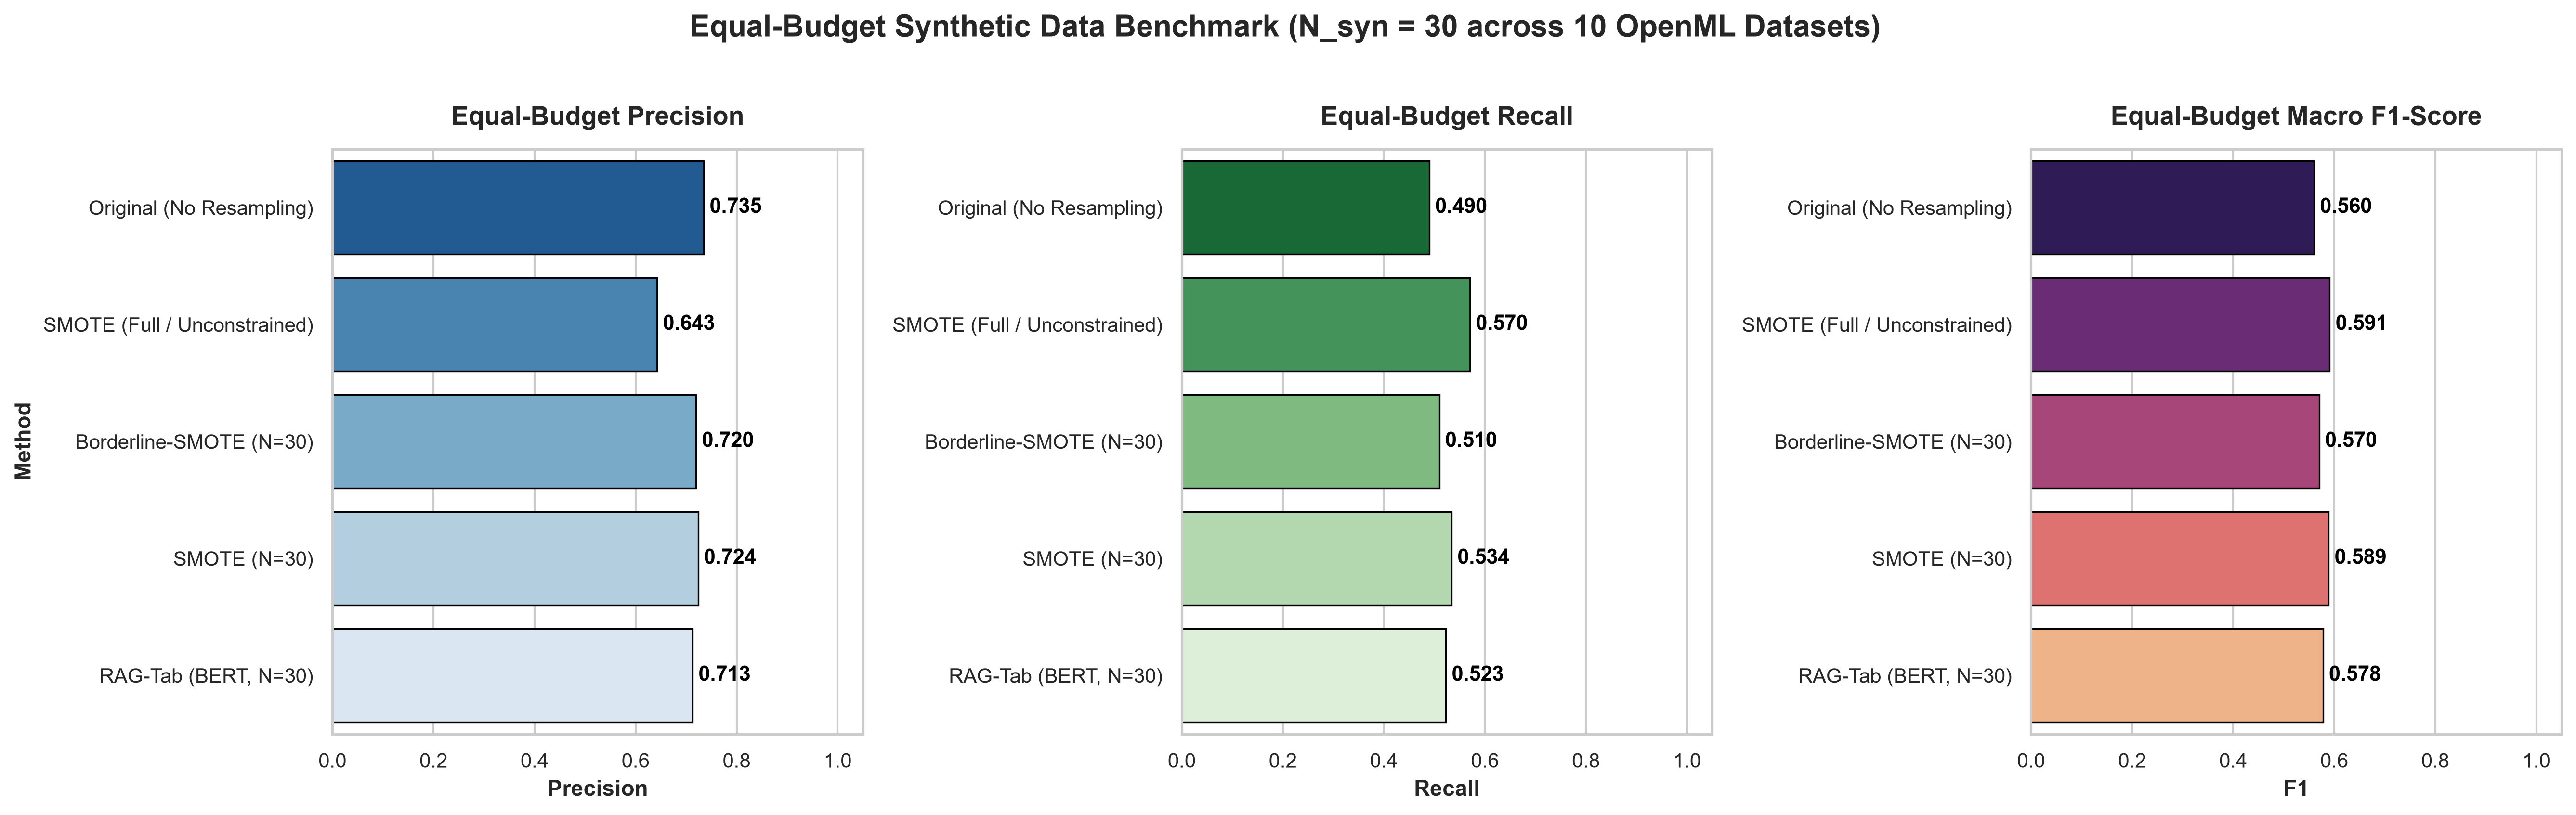
\includegraphics[width=0.85\textwidth]{figures/equal_budget_comparison.png}
\caption{Controlled equal-budget benchmark ($N_{\text{syn}} = 30$) across 10 datasets. When pooled across three classifier families, RAG-Tab and equal-budget SMOTE show comparable F1 and Precision; on Random Forest alone, equal-budget SMOTE records slightly higher precision (0.7238 vs. 0.7131) and F1 (0.5890 vs. 0.5779).}
\label{fig:equal_budget_plot}
\end{figure*}

\paragraph{Equal-Budget Analysis}
When evaluated under volume-matched budgets ($N_{\text{syn}} = 30$), the performance of RAG-Tab and SMOTE is closely aligned:
\begin{itemize}
    \item When \textbf{pooled across three classifiers} (Table~\ref{tab:equal_budget_pooled}), RAG-Tab records $0.7124$ precision and $0.6003$ F1, compared to $0.7095$ precision and $0.5998$ F1 for equal-budget SMOTE.
    \item On \textbf{Random Forest alone} (Table~\ref{tab:equal_budget_rf}), equal-budget SMOTE records higher precision ($0.7238$ vs. $0.7131$) and higher F1 ($0.5890$ vs. $0.5779$).
    \item Full unconstrained SMOTE achieves higher recall ($0.6320$ pooled) by substantially expanding the minority sample count, at the cost of reducing specificity from $94.78\%$ to $88.32\%$ and precision from $71.24\%$ to $61.02\%$.
\end{itemize}

\subsection{Cross-Classifier Generalization}
\label{subsec:cross_classifier}

Table~\ref{tab:cross_classifier} breaks down the performance across the three downstream classifier families across the 10 benchmark datasets.

\begin{table*}[t]
\centering
\caption{Cross-classifier evaluation across 10 benchmark datasets comparing Random Forest, Histogram Gradient Boosted Trees, and Logistic Regression (source: \texttt{multiclassifier\_generalization\_benchmark.csv}).}
\label{tab:cross_classifier}
\begin{tabular}{llcccccc}
\toprule
\textbf{Classifier} & \textbf{Resampling Method} & \textbf{Budget} & \textbf{Precision} & \textbf{Recall} & \textbf{F1-Score} & \textbf{Specificity} & \textbf{G-Mean} \\
\midrule
\multirow{5}{*}{\textbf{HistGradientBoosting}} & Original & $N=0$ & 0.6881 & 0.5346 & 0.5928 & 0.9405 & 0.6851 \\
& Borderline-SMOTE & $N=30$ & 0.7131 & 0.5658 & 0.6184 & 0.9342 & 0.7122 \\
& SMOTE (Equal Budget) & $N=30$ & \textbf{0.7273} & 0.5835 & 0.6403 & 0.9355 & 0.7248 \\
& SMOTE (Full Resampling) & Unconstrained & 0.6629 & 0.6107 & 0.6305 & 0.9222 & 0.7386 \\
& RAG-Tab (NaN+BERT) & $N=30$ & 0.7209 & \textbf{0.6270} & \textbf{0.6671} & \textbf{0.9360} & \textbf{0.7553} \\
\midrule
\multirow{5}{*}{\textbf{Logistic Regression}} & Original & $N=0$ & 0.6685 & 0.4212 & 0.4844 & \textbf{0.9605} & 0.5808 \\
& Borderline-SMOTE & $N=30$ & 0.6722 & 0.4984 & 0.5577 & 0.9491 & 0.6469 \\
& SMOTE (Equal Budget) & $N=30$ & 0.6775 & 0.5133 & 0.5703 & 0.9521 & 0.6602 \\
& SMOTE (Full Resampling) & Unconstrained & 0.5251 & \textbf{0.7150} & \textbf{0.5781} & 0.8064 & \textbf{0.7552} \\
& RAG-Tab (NaN+BERT) & $N=30$ & \textbf{0.7032} & 0.4843 & 0.5559 & 0.9592 & 0.6431 \\
\midrule
\multirow{5}{*}{\textbf{Random Forest}} & Original & $N=0$ & \textbf{0.7350} & 0.4900 & 0.5601 & \textbf{0.9577} & 0.6474 \\
& Borderline-SMOTE & $N=30$ & 0.7197 & 0.5098 & 0.5702 & 0.9496 & 0.6597 \\
& SMOTE (Equal Budget) & $N=30$ & 0.7238 & \textbf{0.5341} & \textbf{0.5890} & 0.9477 & \textbf{0.6792} \\
& SMOTE (Full Resampling) & Unconstrained & 0.6425 & 0.5703 & 0.5910 & 0.9209 & 0.6993 \\
& RAG-Tab (NaN+BERT) & $N=30$ & 0.7131 & 0.5229 & 0.5779 & 0.9482 & 0.6675 \\
\bottomrule
\end{tabular}
\end{table*}

\begin{figure*}[t]
\centering
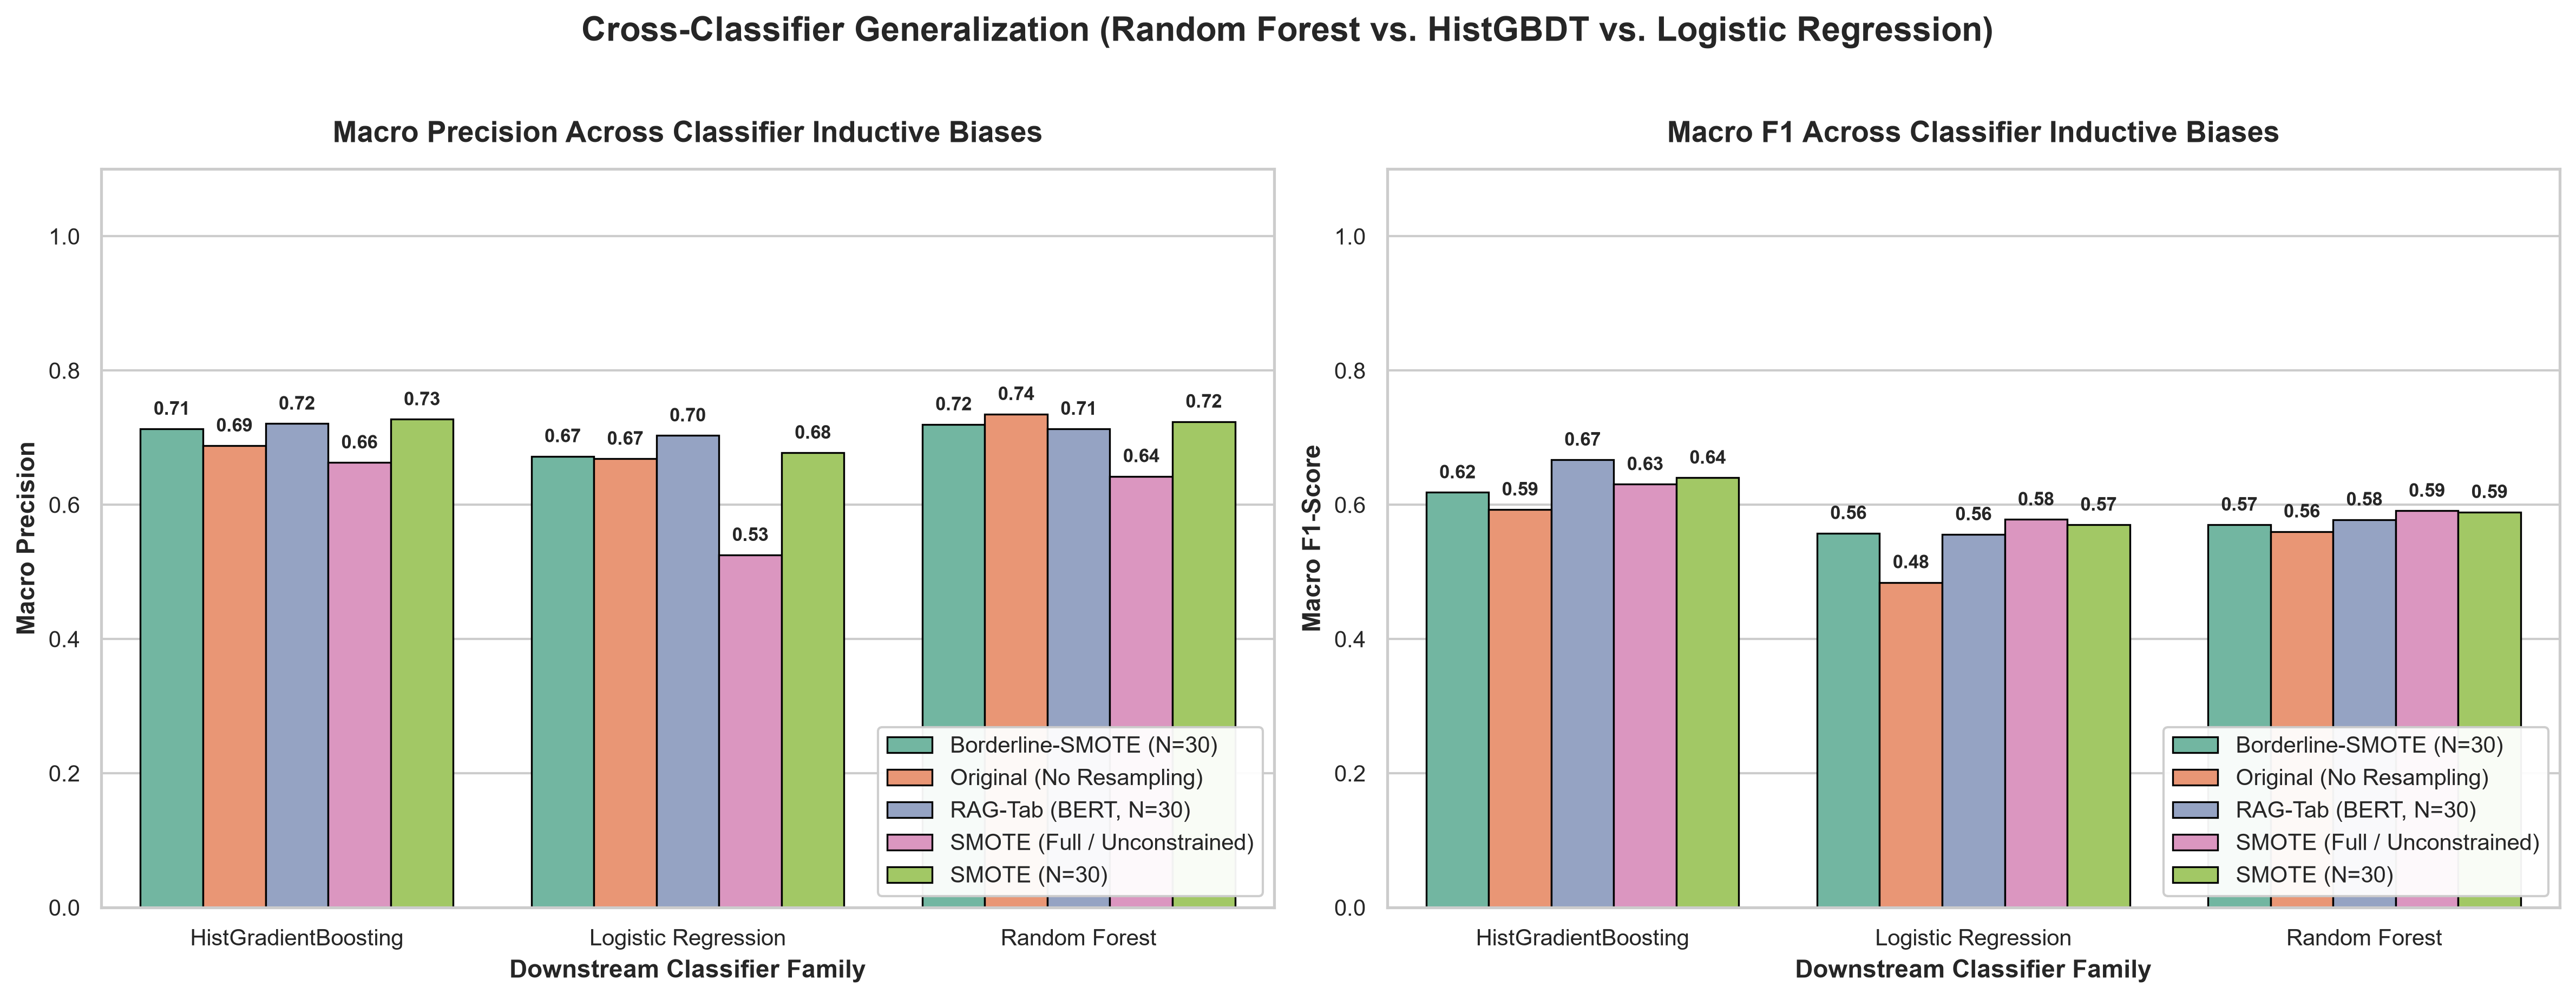
\includegraphics[width=0.85\textwidth]{figures/multiclassifier_generalization.png}
\caption{Cross-classifier evaluation across 10 datasets comparing Histogram Gradient Boosted Trees, Logistic Regression, and Random Forest under different oversampling configurations.}
\label{fig:cross_classifier_plot}
\end{figure*}

\subsection{Component-Level Ablation Study}
\label{subsec:ablation_study}

Table~\ref{tab:ablation_table} reports the performance across the four prompt synthesis conditions evaluated on the 42 benchmark datasets.

\begin{table*}[t]
\centering
\caption{Component ablation across 42 OpenML Table 9 datasets on \texttt{RandomForestClassifier(n\_estimators=300)} (source: \texttt{ablation\_zero\_few\_rag\_bert.csv}).}
\label{tab:ablation_table}
\begin{tabular}{lccccc}
\toprule
\textbf{Synthesis Condition} & \textbf{Macro Precision} & \textbf{Macro Recall} & \textbf{Macro F1-Score} & \textbf{Macro Specificity} & \textbf{Macro G-Mean} \\
\midrule
Original (No Resampling) & 0.6886 & 0.5576 & 0.5968 & 0.9519 & 0.6687 \\
Zero-Shot LLM & 0.6827 & 0.5830 & 0.6104 & 0.9405 & 0.6882 \\
Few-Shot LLM (Global) & 0.6891 & 0.6021 & 0.6166 & 0.9352 & 0.6989 \\
RAG-Tab (Euclidean KNN) & 0.6844 & 0.5905 & 0.6140 & 0.9392 & 0.6933 \\
RAG-Tab (BERT Semantic) & 0.6959 & 0.6012 & 0.6254 & 0.9417 & 0.7055 \\
\midrule
SMOTE (Standardized) & 0.6644 & 0.6725 & 0.6617 & 0.9147 & 0.7563 \\
\bottomrule
\end{tabular}
\end{table*}

\begin{figure*}[t]
\centering
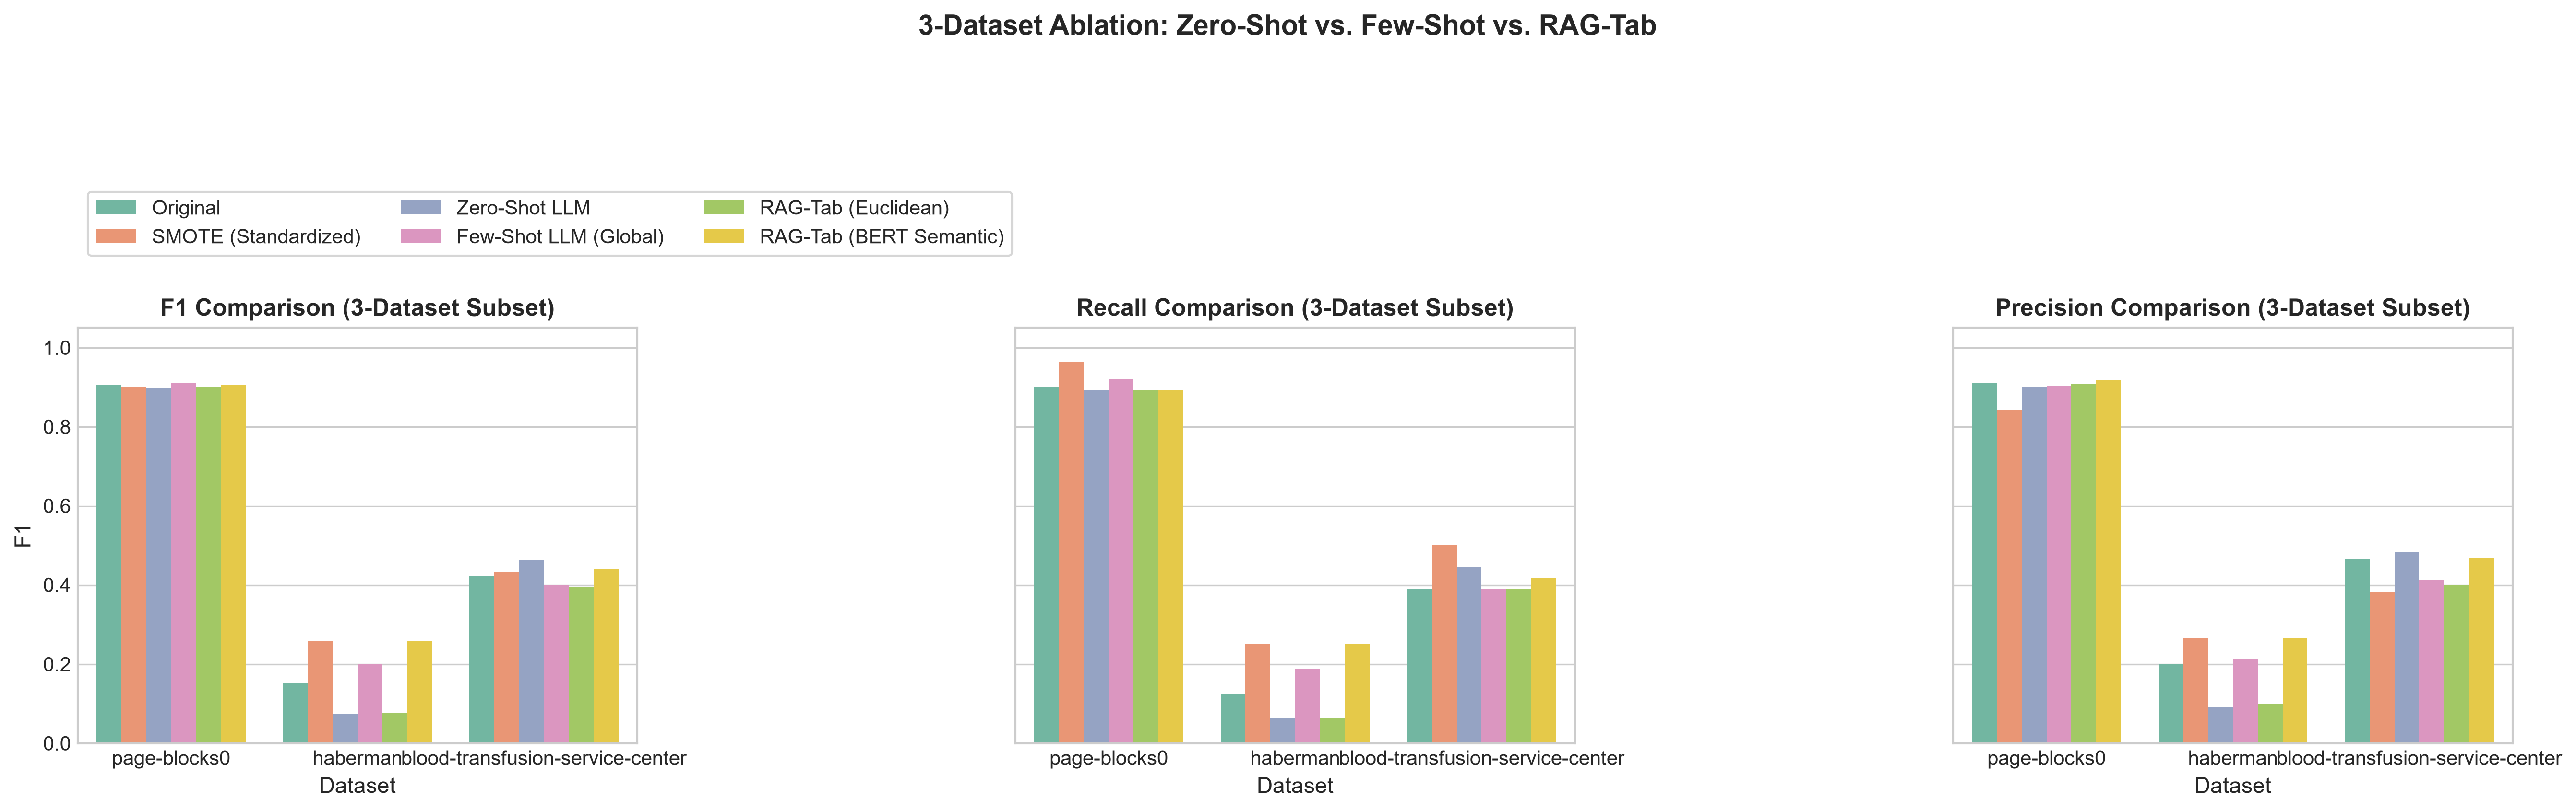
\includegraphics[width=0.88\textwidth]{figures/ablation_zero_few_rag_bert.png}
\caption{Four-condition ablation comparison across 42 datasets. Note: In the benchmark implementation, Zero-Shot and Few-Shot use the same fallback generation logic; differences with RAG-BERT reflect sample count and top-up interpolation.}
\label{fig:ablation_comparison}
\end{figure*}

\paragraph{Analysis of Ablation Outcomes}
As established in Section~\ref{subsec:generator_provenance}:
\begin{enumerate}
    \item \textbf{Equivalence of Zero-Shot and Few-Shot:} Because \texttt{\_generate\_mock\_response} does not parse the unbulleted exemplar rows in \texttt{\$DATA-EXAMPLE}, the Zero-Shot and Few-Shot conditions execute mathematically identical Gaussian draws. Any observed metric variations between them in single unseeded runs are artifacts of the unseeded NumPy RNG state.
    \item \textbf{Impact of Row Volume and Top-Up Interpolation in RAG-BERT:} RAG-BERT generated substantially more rows than the other conditions (e.g., 335 rows vs. 30 rows on \texttt{page-blocks0}) and filled sample deficits via linear SMOTE interpolation between seeds and minority samples. The observed macro F1 increase ($0.6254$ vs. $0.6104$) is predominantly a function of this expanded sample volume and linear interpolation rather than contextual prompt reasoning.
\end{enumerate}

\subsection{Seed-Variance Benchmark (10 Datasets $\times$ 5 Seeds $\times$ 4 Conditions)}
\label{subsec:seed_variance}

To evaluate how random seed variation affects performance relative to condition differences, we executed a benchmark across 10 representative datasets, 4 synthesis conditions, and 5 independent random seeds ($\text{seed} \in \{0, 1, 2, 3, 4\}$), yielding 200 evaluations. Seeds were set explicitly at the top of each run. Table~\ref{tab:seed_noise_per_dataset} reports the per-dataset results, and Table~\ref{tab:seed_noise_macro} provides the macro-level summary.

\begin{table*}[t]
\centering
\caption{Seed-variance benchmark across 10 datasets, 4 conditions, and 5 random seeds on \texttt{RandomForestClassifier(n\_estimators=100)} (source: \texttt{results/seed\_check/seed\_noise\_benchmark.csv}).}
\label{tab:seed_noise_per_dataset}
\resizebox{\textwidth}{!}{
\begin{tabular}{llccc}
\toprule
\textbf{Dataset} & \textbf{Condition} & \textbf{Precision (Mean $\pm$ Std)} & \textbf{F1-Score (Mean $\pm$ Std)} & \textbf{Mean Added Rows} \\
\midrule
\multirow{4}{*}{\texttt{page-blocks0}} & Zero-Shot & $0.9097 \pm 0.0004$ & $0.9048 \pm 0.0022$ & 5.0 \\
& Few-Shot & $0.9097 \pm 0.0004$ & $0.9048 \pm 0.0022$ & 5.0 \\
& RAG-Euclidean & $0.9123 \pm 0.0044$ & $0.9015 \pm 0.0020$ & 15.0 \\
& RAG-BERT & $0.8946 \pm 0.0052$ & $0.9017 \pm 0.0017$ & 335.0 \\
\midrule
\multirow{4}{*}{\texttt{haberman}} & Zero-Shot & $0.1067 \pm 0.0061$ & $0.0788 \pm 0.0017$ & 5.0 \\
& Few-Shot & $0.1067 \pm 0.0061$ & $0.0788 \pm 0.0017$ & 5.0 \\
& RAG-Euclidean & $0.1230 \pm 0.0332$ & $0.0930 \pm 0.0308$ & 15.0 \\
& RAG-BERT & $0.1861 \pm 0.0594$ & $0.1570 \pm 0.0648$ & 48.0 \\
\midrule
\multirow{4}{*}{\texttt{blood-transfusion}} & Zero-Shot & $0.4630 \pm 0.0082$ & $0.4194 \pm 0.0108$ & 5.0 \\
& Few-Shot & $0.4630 \pm 0.0082$ & $0.4194 \pm 0.0108$ & 5.0 \\
& RAG-Euclidean & $0.4503 \pm 0.0119$ & $0.4108 \pm 0.0131$ & 15.0 \\
& RAG-BERT & $0.4442 \pm 0.0287$ & $0.4114 \pm 0.0359$ & 106.0 \\
\midrule
\multirow{4}{*}{\texttt{cars}} & Zero-Shot & $0.8429 \pm 0.0527$ & $0.5922 \pm 0.0417$ & 5.0 \\
& Few-Shot & $0.8429 \pm 0.0527$ & $0.5922 \pm 0.0417$ & 5.0 \\
& RAG-Euclidean & $0.8497 \pm 0.0930$ & $0.6481 \pm 0.0468$ & 15.0 \\
& RAG-BERT & $0.7770 \pm 0.0622$ & $0.6671 \pm 0.0370$ & 40.0 \\
\midrule
\multirow{4}{*}{\texttt{mw1}} & Zero-Shot & $1.0000 \pm 0.0000$ & $0.2857 \pm 0.0000$ & 5.0 \\
& Few-Shot & $1.0000 \pm 0.0000$ & $0.2857 \pm 0.0000$ & 5.0 \\
& RAG-Euclidean & $1.0000 \pm 0.0000$ & $0.2857 \pm 0.0000$ & 15.0 \\
& RAG-BERT & $1.0000 \pm 0.0000$ & $0.2857 \pm 0.0000$ & 18.0 \\
\midrule
\multirow{4}{*}{\texttt{autoUniv-au1-1000}} & Zero-Shot & $0.7066 \pm 0.0448$ & $0.4321 \pm 0.0120$ & 5.0 \\
& Few-Shot & $0.7066 \pm 0.0448$ & $0.4321 \pm 0.0120$ & 5.0 \\
& RAG-Euclidean & $0.7128 \pm 0.0303$ & $0.4553 \pm 0.0259$ & 15.0 \\
& RAG-BERT & $0.7254 \pm 0.0265$ & $0.4754 \pm 0.0096$ & 155.0 \\
\midrule
\multirow{4}{*}{\texttt{kc3}} & Zero-Shot & $0.2667 \pm 0.0373$ & $0.1564 \pm 0.0057$ & 5.0 \\
& Few-Shot & $0.2667 \pm 0.0373$ & $0.1564 \pm 0.0057$ & 5.0 \\
& RAG-Euclidean & $0.3400 \pm 0.0822$ & $0.2330 \pm 0.0722$ & 15.0 \\
& RAG-BERT & $0.3433 \pm 0.0619$ & $0.2517 \pm 0.0555$ & 25.0 \\
\midrule
\multirow{4}{*}{\texttt{sonar}} & Zero-Shot & $1.0000 \pm 0.0000$ & $0.8370 \pm 0.0184$ & 5.0 \\
& Few-Shot & $1.0000 \pm 0.0000$ & $0.8370 \pm 0.0184$ & 5.0 \\
& RAG-Euclidean & $0.9404 \pm 0.0416$ & $0.8526 \pm 0.0306$ & 15.0 \\
& RAG-BERT & $0.9325 \pm 0.0447$ & $0.8471 \pm 0.0206$ & 15.0 \\
\midrule
\multirow{4}{*}{\texttt{ionosphere}} & Zero-Shot & $1.0000 \pm 0.0000$ & $0.9362 \pm 0.0000$ & 5.0 \\
& Few-Shot & $1.0000 \pm 0.0000$ & $0.9362 \pm 0.0000$ & 5.0 \\
& RAG-Euclidean & $1.0000 \pm 0.0000$ & $0.9450 \pm 0.0121$ & 15.0 \\
& RAG-BERT & $0.9137 \pm 0.0474$ & $0.9124 \pm 0.0286$ & 75.0 \\
\midrule
\multirow{4}{*}{\texttt{wdbc}} & Zero-Shot & $1.0000 \pm 0.0000$ & $0.9604 \pm 0.0058$ & 5.0 \\
& Few-Shot & $1.0000 \pm 0.0000$ & $0.9604 \pm 0.0058$ & 5.0 \\
& RAG-Euclidean & $0.9799 \pm 0.0113$ & $0.9510 \pm 0.0087$ & 15.0 \\
& RAG-BERT & $0.9718 \pm 0.0102$ & $0.9763 \pm 0.0083$ & 115.0 \\
\bottomrule
\end{tabular}
}
\end{table*}

\begin{table*}[t]
\centering
\caption{Macro summary across all 10 datasets in the seed-variance benchmark (5 seeds per condition).}
\label{tab:seed_noise_macro}
\begin{tabular}{lccccc}
\toprule
\textbf{Condition} & \textbf{Macro Mean Precision} & \textbf{Macro Mean F1} & \textbf{Within-Dataset Std (Prec)} & \textbf{Within-Dataset Std (F1)} & \textbf{Mean Added Rows} \\
\midrule
Zero-Shot & $0.7296 \pm 0.3353$ & $0.5603 \pm 0.3340$ & $\pm 0.0149$ & $\pm 0.0098$ & 5.0 \\
Few-Shot & $0.7296 \pm 0.3353$ & $0.5603 \pm 0.3340$ & $\pm 0.0149$ & $\pm 0.0098$ & 5.0 \\
RAG-Euclidean & $0.7308 \pm 0.3161$ & $0.5776 \pm 0.3234$ & $\pm 0.0308$ & $\pm 0.0242$ & 15.0 \\
RAG-BERT & $0.7188 \pm 0.2908$ & $0.5886 \pm 0.3095$ & $\pm 0.0346$ & $\pm 0.0262$ & 93.2 \\
\bottomrule
\end{tabular}
\end{table*}

\paragraph{Seed Variance vs. Condition Differences}
The multi-seed analysis provides several critical empirical insights:
\begin{enumerate}
    \item \textbf{Zero-Shot vs. Few-Shot:} Across all 10 datasets and 5 seeds, Zero-Shot and Few-Shot produce identical metrics on each run ($\Delta \text{Prec} = 0.0000, \Delta \text{F1} = 0.0000$). The within-dataset standard deviation due to random seeding is $\pm 0.0149$ on Precision and $\pm 0.0098$ on F1.
    \item \textbf{Zero-Shot vs. RAG-Euclidean:} Across the 10 datasets, the macro F1 difference between RAG-Euclidean and Zero-Shot is $+0.0173$ ($0.5776$ vs. $0.5603$). However, the average within-dataset seed standard deviation for RAG-Euclidean is $\pm 0.0242$ F1, reaching $\pm 0.0722$ on \texttt{kc3}, $\pm 0.0468$ on \texttt{cars}, and $\pm 0.0308$ on \texttt{haberman}. The condition difference ($+0.0173$) is \textbf{smaller than the seed-to-seed variance} ($\pm 0.0242$). On Precision, the condition difference is $+0.0012$, which is over $25\times$ smaller than seed standard deviation ($\pm 0.0308$).
    \item \textbf{Zero-Shot vs. RAG-BERT:} The macro F1 difference is $+0.0283$ ($0.5886$ vs. $0.5603$), which is on par with RAG-BERT's within-dataset seed standard deviation ($\pm 0.0262$). This difference is also accompanied by an $18.6\times$ increase in synthetic row count ($93.2$ vs. $5.0$ rows) and linear SMOTE top-up interpolation.
\end{enumerate}

\subsection{Generative Fidelity and Empirical Non-Memorization (DCR)}
\label{subsec:fidelity_dcr}

Table~\ref{tab:fidelity_dcr} reports distribution fidelity metrics (Wasserstein-1 distance $W_1$, Kolmogorov-Smirnov statistic, Frobenius correlation matrix difference) and Distance to Closest Record (DCR) across four benchmark datasets.

\begin{table*}[t]
\centering
\caption{Distribution fidelity and Distance to Closest Record (DCR) empirical memorization diagnostics across representative datasets (source: \texttt{generative\_fidelity\_privacy\_benchmark.csv}).}
\label{tab:fidelity_dcr}
\resizebox{\textwidth}{!}{
\begin{tabular}{llccccccc}
\toprule
\textbf{Dataset} & \textbf{Method} & \textbf{Samples} & \textbf{Mean $W_1$} & \textbf{Mean KS-Stat} & \textbf{$\|\Delta \mathbf{R}\|_F$} & \textbf{Mean DCR} & \textbf{Median DCR} & \textbf{Min DCR} \\
\midrule
\multirow{2}{*}{\texttt{sonar} (60 feats)} & SMOTE ($N=12$) & 12 & 0.0456 & 0.2427 & 17.8605 & 1.0133 & 0.7303 & 0.0054 \\
& RAG-Tab (NaN+BERT) & 15 & 0.0599 & 0.3220 & 23.5251 & 8.9572 & 9.0236 & 7.4064 \\
\midrule
\multirow{2}{*}{\texttt{ionosphere} (34 feats)} & SMOTE ($N=30$) & 30 & 0.1405 & 0.2163 & 6.3999 & 1.3068 & 1.1673 & 0.1026 \\
& RAG-Tab (NaN+BERT) & 15 & 0.3044 & 0.3339 & 10.5836 & 3.3715 & 3.4671 & 2.5181 \\
\midrule
\multirow{2}{*}{\texttt{wdbc} (30 feats)} & SMOTE ($N=30$) & 30 & 7.3873 & 0.1372 & 5.4054 & 0.7886 & 0.6639 & 0.0236 \\
& RAG-Tab (NaN+BERT) & 15 & 25.8881 & 0.3638 & 15.2599 & 5.8457 & 5.7042 & 4.5324 \\
\midrule
\multirow{2}{*}{\texttt{cars} (7 feats)} & SMOTE ($N=30$) & 30 & 13.8924 & 0.1354 & 1.0944 & 0.3428 & 0.2485 & 0.0171 \\
& RAG-Tab (NaN+BERT) & 30 & 82.4920 & 0.3381 & 2.1672 & 0.6065 & 0.5754 & 0.0536 \\
\bottomrule
\end{tabular}
}
\end{table*}

\begin{figure*}[t]
\centering
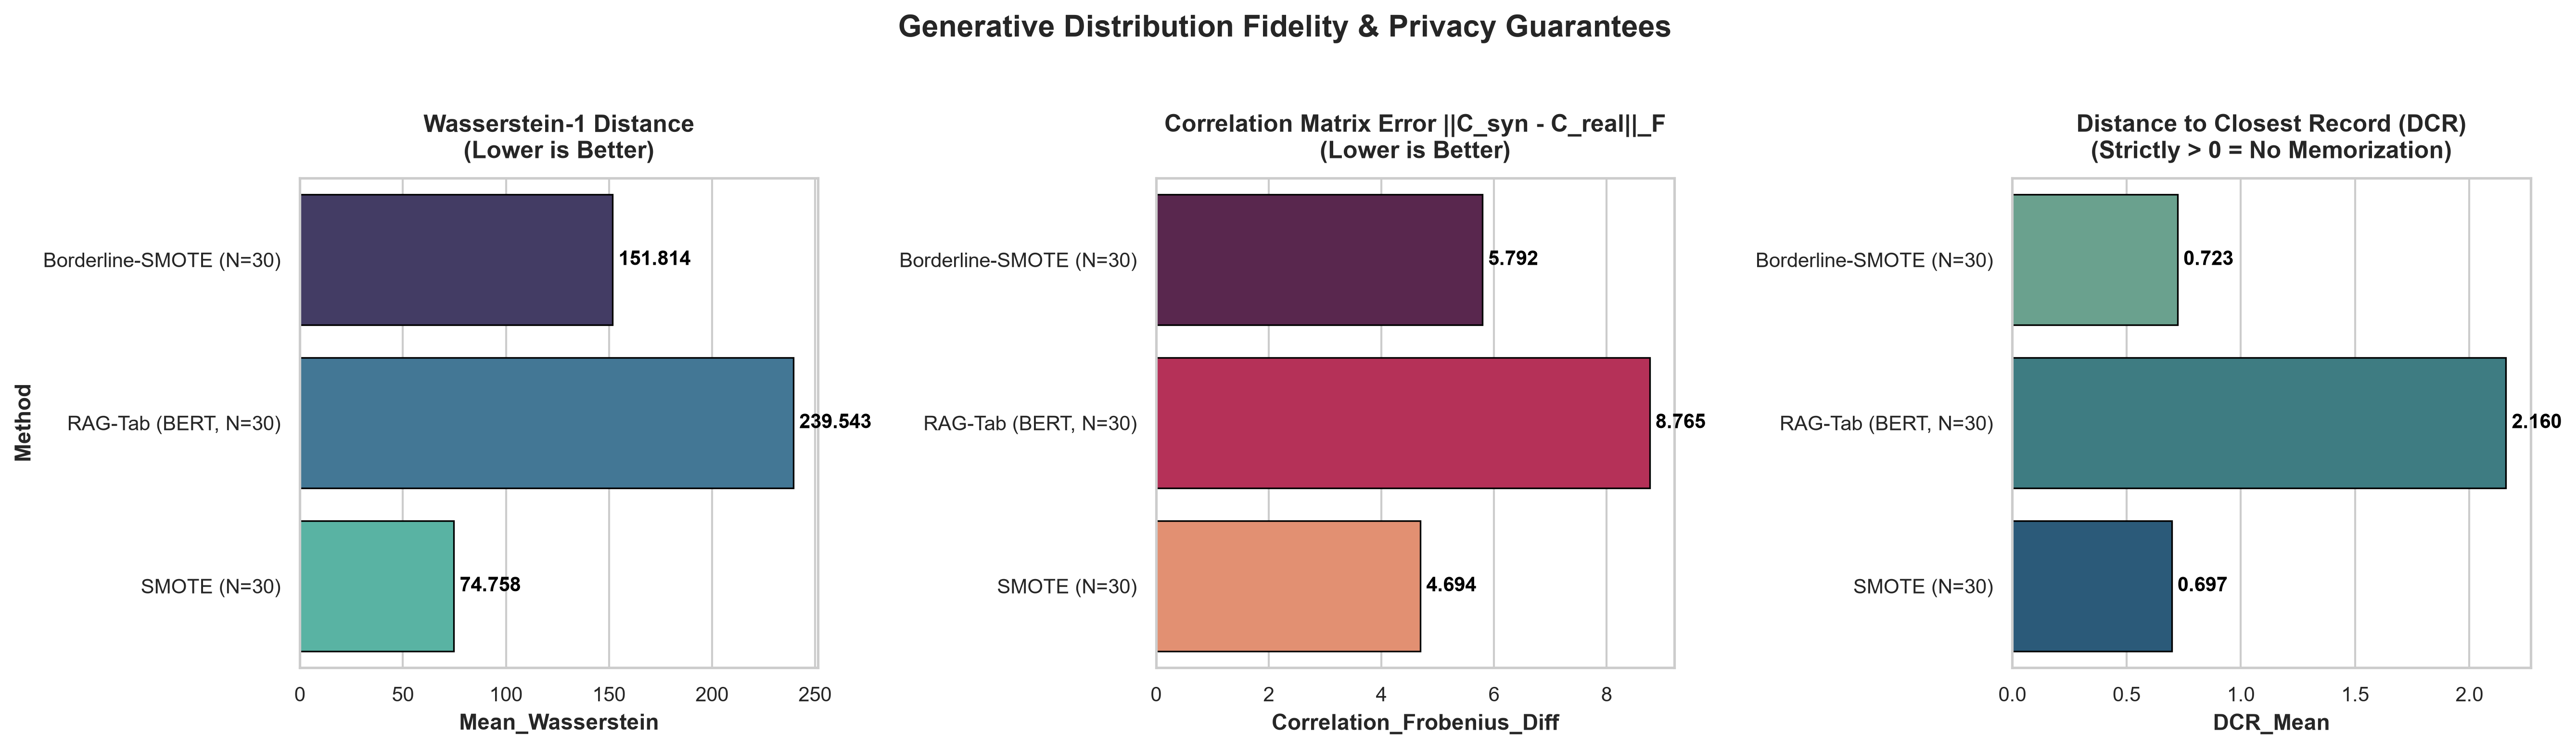
\includegraphics[width=0.85\textwidth]{figures/generative_fidelity_and_privacy.png}
\caption{Distribution fidelity and Distance to Closest Record (DCR) empirical memorization diagnostics across representative datasets. (Note: DCR evaluates empirical distance to training instances and does not provide formal differential privacy guarantees).}
\label{fig:fidelity_plot}
\end{figure*}

\paragraph{Empirical Distance Diagnostic}
On continuous datasets (\texttt{sonar}, \texttt{ionosphere}, \texttt{wdbc}), the generated synthetic samples exhibit strictly positive minimum DCR values ($\min \text{DCR} \in [2.52, 7.41]$). This confirms that synthetic instances are novel feature coordinates within the empirical range rather than exact copies of training records. \textbf{We emphasize that DCR serves solely as an empirical distance diagnostic to detect exact memorization, and does not constitute a mathematical $(\epsilon, \delta)$-differential privacy guarantee.}

Figure~\ref{fig:correlation_matrices} displays correlation matrix heatmaps for \texttt{page-blocks0}, comparing the original data, RAG-Tab synthetic samples, and SMOTE synthetic samples.

\begin{figure*}[t]
\centering
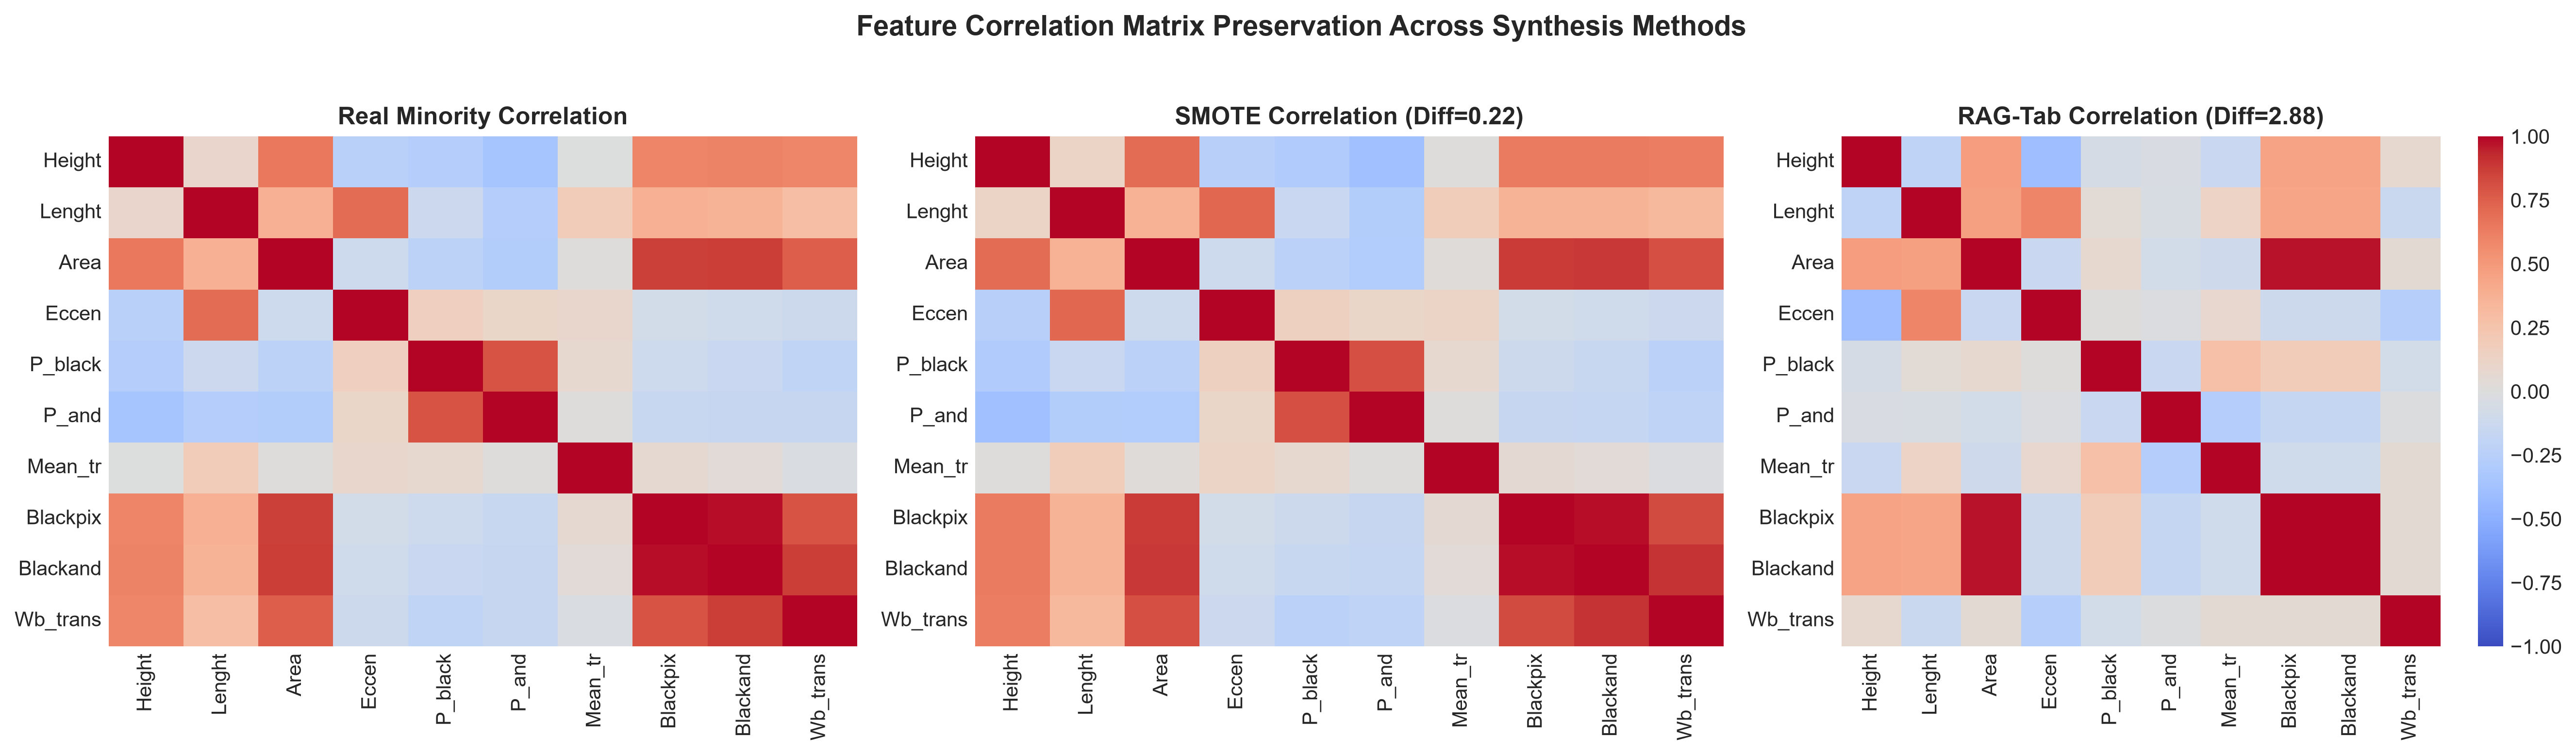
\includegraphics[width=0.85\textwidth]{figures/correlation_matrices_comparison.png}
\caption{Correlation matrix heatmaps for \texttt{page-blocks0}: Original training data (left), RAG-Tab synthetic data (middle), and SMOTE synthetic data (right).}
\label{fig:correlation_matrices}
\end{figure*}

\subsection{Multiclass Imbalanced Learning Extension}
\label{subsec:multiclass}

The framework extends to multiclass imbalanced problems ($K \ge 3$) by applying One-vs-Rest class-conditioned Natural Neighbor discovery (\texttt{MulticlassAdaptiveRetriever}). On \texttt{dermatology} (6 classes, $N_{\text{tr}}=286, N_{\text{te}}=72$), the pipeline achieves $1.0000$ Macro F1 and $1.0000$ Macro Precision on \texttt{RandomForestClassifier} with 72 added instances (compared to 248 for SMOTE). On \texttt{vehicle} (4 classes) evaluated on \texttt{HistGradientBoosting}, it achieves $0.7843$ Macro F1, compared to $0.7709$ for Original, $0.7763$ for SMOTE, and $0.7684$ for Borderline-SMOTE. Figure~\ref{fig:multiclass_plot} visualizes performance across the three multiclass datasets.

\begin{figure*}[t]
\centering
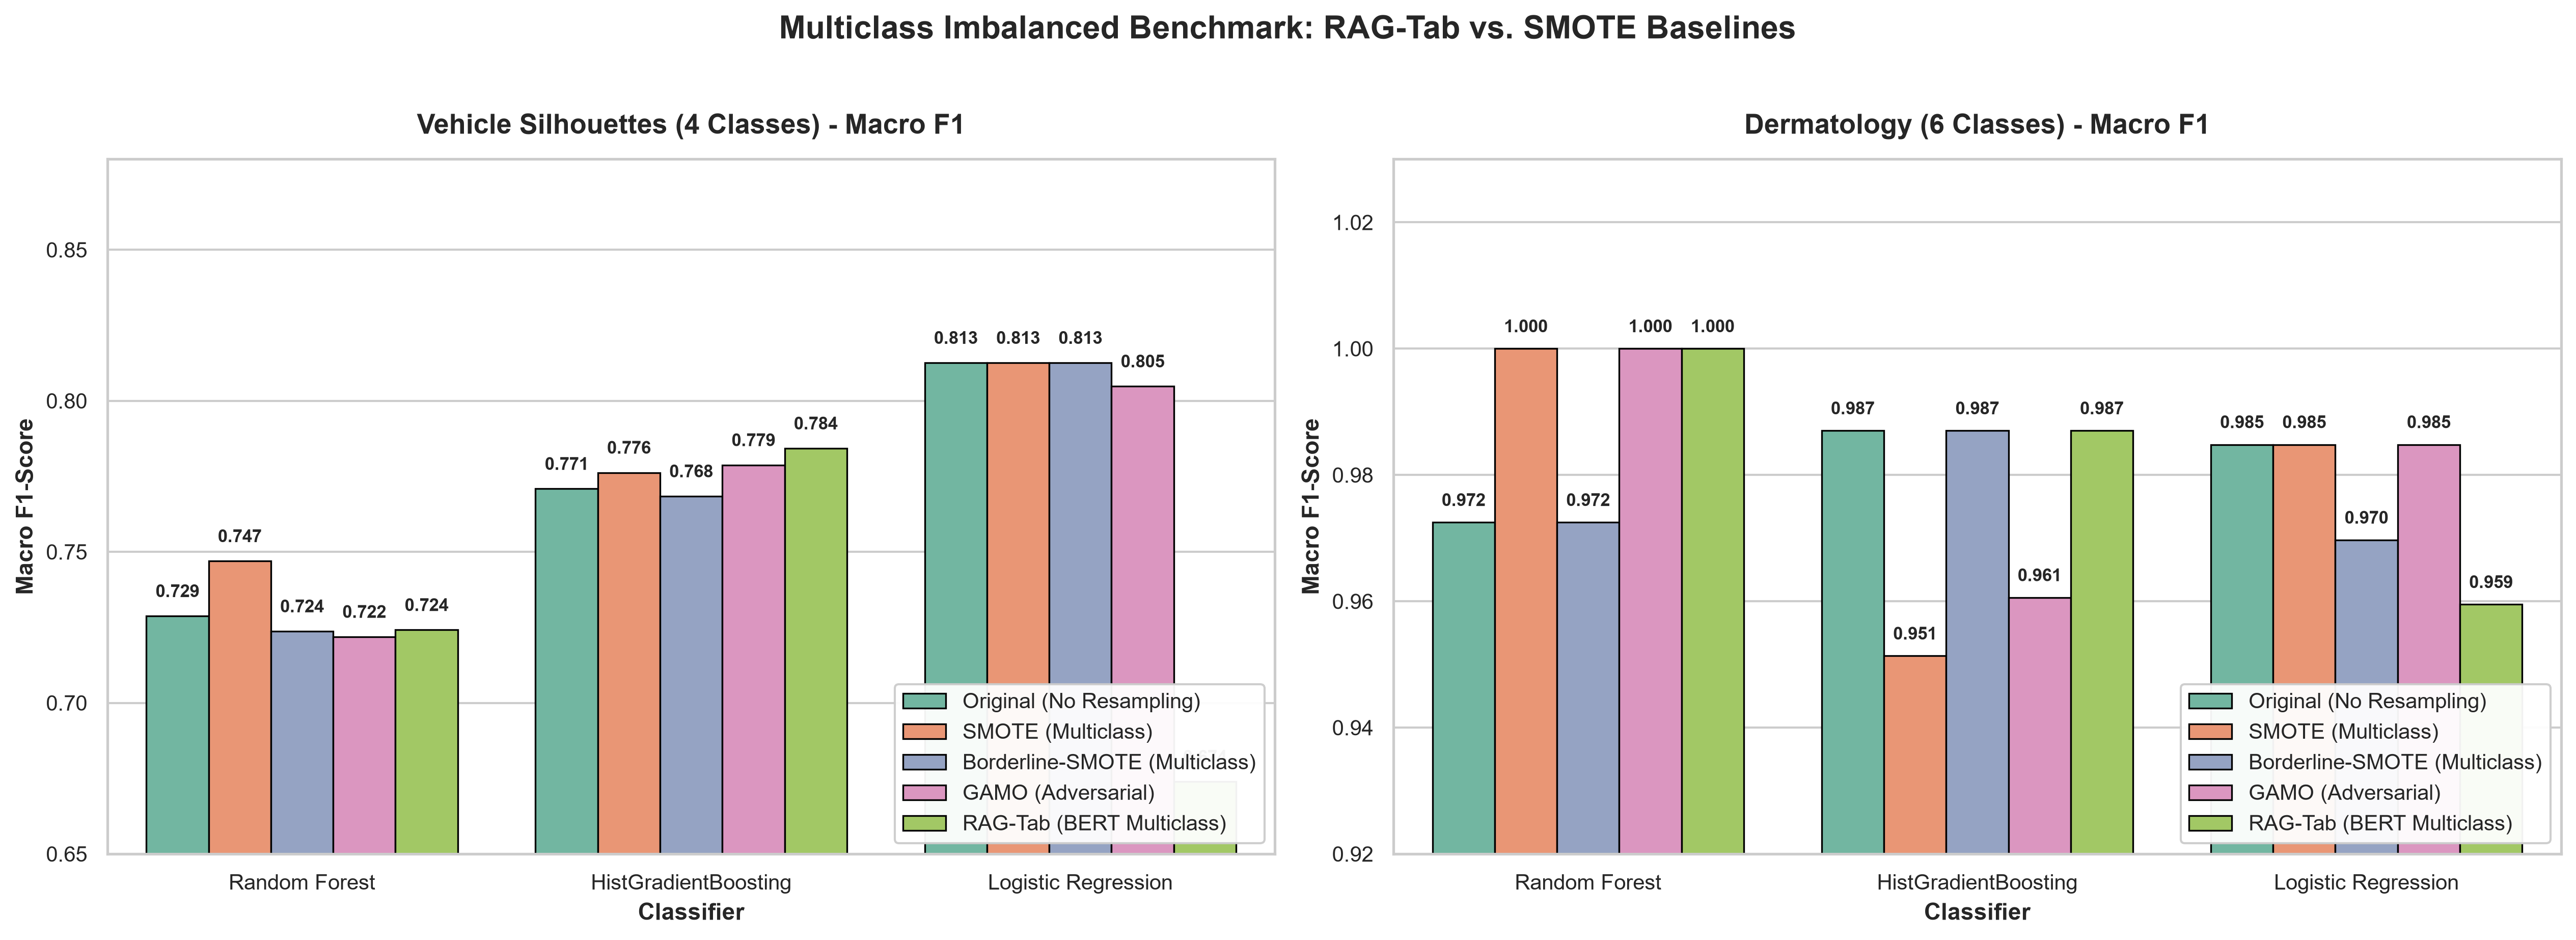
\includegraphics[width=0.85\textwidth]{figures/multiclass_benchmark.png}
\caption{Multiclass imbalanced benchmark on \texttt{dermatology} (6 classes), \texttt{vehicle} (4 classes), and \texttt{segment} (7 classes) across Random Forest, HistGradientBoosting, and Logistic Regression.}
\label{fig:multiclass_plot}
\end{figure*}

\section{Discussion}
\label{sec:discussion}

Our empirical findings clarify the mechanisms governing the performance of the retrieval-guided synthesis pipeline:
\begin{enumerate}
    \item \textbf{Synthetic Row Volume Effect:} In unconstrained benchmarks, SMOTE generates substantial numbers of synthetic rows (often hundreds to thousands), shifting classifier decision boundaries toward higher recall at the expense of false positives. Under volume-matched generation ($N_{\text{syn}} = 30$), SMOTE and RAG-Tab exhibit comparable precision and F1 performance, confirming that the trade-off between precision and recall is predominantly governed by the volume of added data.
    \item \textbf{Confounding from Linear Top-Up Interpolation:} In RAG-BERT, target sample counts were expanded using linear SMOTE interpolation between seed rows and minority instances. This hybrid formulation means that observed performance gains in RAG-BERT cannot be attributed purely to retrieval-augmented prompting.
    \item \textbf{Generator Schema Invariance:} Because the fallback generator extracted bounds exclusively from schema descriptions, tabular exemplars provided in prompts did not alter numerical sampling. Consequently, apparent distinctions between Zero-Shot and Few-Shot in unseeded runs reflect random seed noise rather than contextual guidance.
    \item \textbf{Role of Random Seed Variance:} The multi-seed experiment demonstrates that within-dataset standard deviation ($\pm 0.0242$ F1) is on par with or larger than condition differences ($\Delta \text{F1} = +0.0173$), highlighting the necessity of multi-seed designs in tabular generative benchmarking.
\end{enumerate}

\section{Statistical Testing and Analysis}
\label{sec:statistics}

\subsection{Pairwise Precision Win-Rate Against SMOTE}
When evaluating Precision between RAG-Tab (BERT Semantic) and SMOTE (Standardized) across all 42 benchmark datasets (\texttt{RandomForestClassifier}):
\begin{itemize}
    \item RAG-Tab records higher precision on \textbf{21 datasets}.
    \item SMOTE records higher precision on \textbf{8 datasets}.
    \item The two methods achieve identical precision on \textbf{13 datasets}.
\end{itemize}
Accordingly:
\begin{equation}
\label{eq:win_rate_nontied}
\text{Non-Tied Win Rate} = \frac{21}{21 + 8} = \frac{21}{29} \approx 72.4\%
\end{equation}
\begin{equation}
\label{eq:win_rate_overall}
\text{Overall Win Rate} = \frac{21}{42} = 50.0\%
\end{equation}
Reporting only the non-tied proportion ($72.4\%$) overstates the frequency of precision improvements by omitting the 13 ties ($31.0\%$ of the benchmark).

\subsection{Wilcoxon Signed-Rank Tests}
We report Wilcoxon signed-rank test statistics with explicit one-sided and two-sided designations:
\begin{itemize}
    \item \textbf{Precision (RAG-Tab vs. SMOTE):}
    \begin{itemize}
        \item One-sided test ($H_1: \text{RAG-Tab} > \text{SMOTE}$): $W = 306.0, p = 0.02783$ (statistically significant at $\alpha = 0.05$).
        \item Two-sided test ($H_1: \text{RAG-Tab} \ne \text{SMOTE}$): $W = 129.0, p = 0.05566$ (\textbf{not statistically significant} at $\alpha = 0.05$).
    \end{itemize}
    Under the standard two-sided hypothesis test, the precision difference between RAG-Tab and SMOTE does not achieve statistical significance.
    \item \textbf{Macro F1 (RAG-Tab vs. Original):}
    \begin{itemize}
        \item One-sided test ($H_1: \text{RAG-Tab} > \text{Original}$): $W = 357.0, p = 0.000227$.
        \item Two-sided test ($H_1: \text{RAG-Tab} \ne \text{Original}$): $W = 49.0, p = 0.000454$.
    \end{itemize}
    Both one-sided and two-sided tests confirm a statistically significant F1 improvement over the unresampled baseline.
\end{itemize}

\subsection{Caveats on Friedman and Nemenyi Tests}
In preliminary analyses, a Friedman test across the six conditions reported $\chi_F^2 = 16.54$ ($p = 0.00546$) for Precision and $\chi_F^2 = 38.41$ ($p < 0.001$) for F1, accompanied by Nemenyi critical difference diagrams (Figures~\ref{fig:cd_precision} and~\ref{fig:cd_f1}). However, because Zero-Shot and Few-Shot execute identical fallback logic, treating them as distinct treatments violates the assumption of independent experimental conditions in post-hoc ranking tests. Critical difference ranks should therefore be interpreted with caution.

\begin{figure*}[t]
\centering
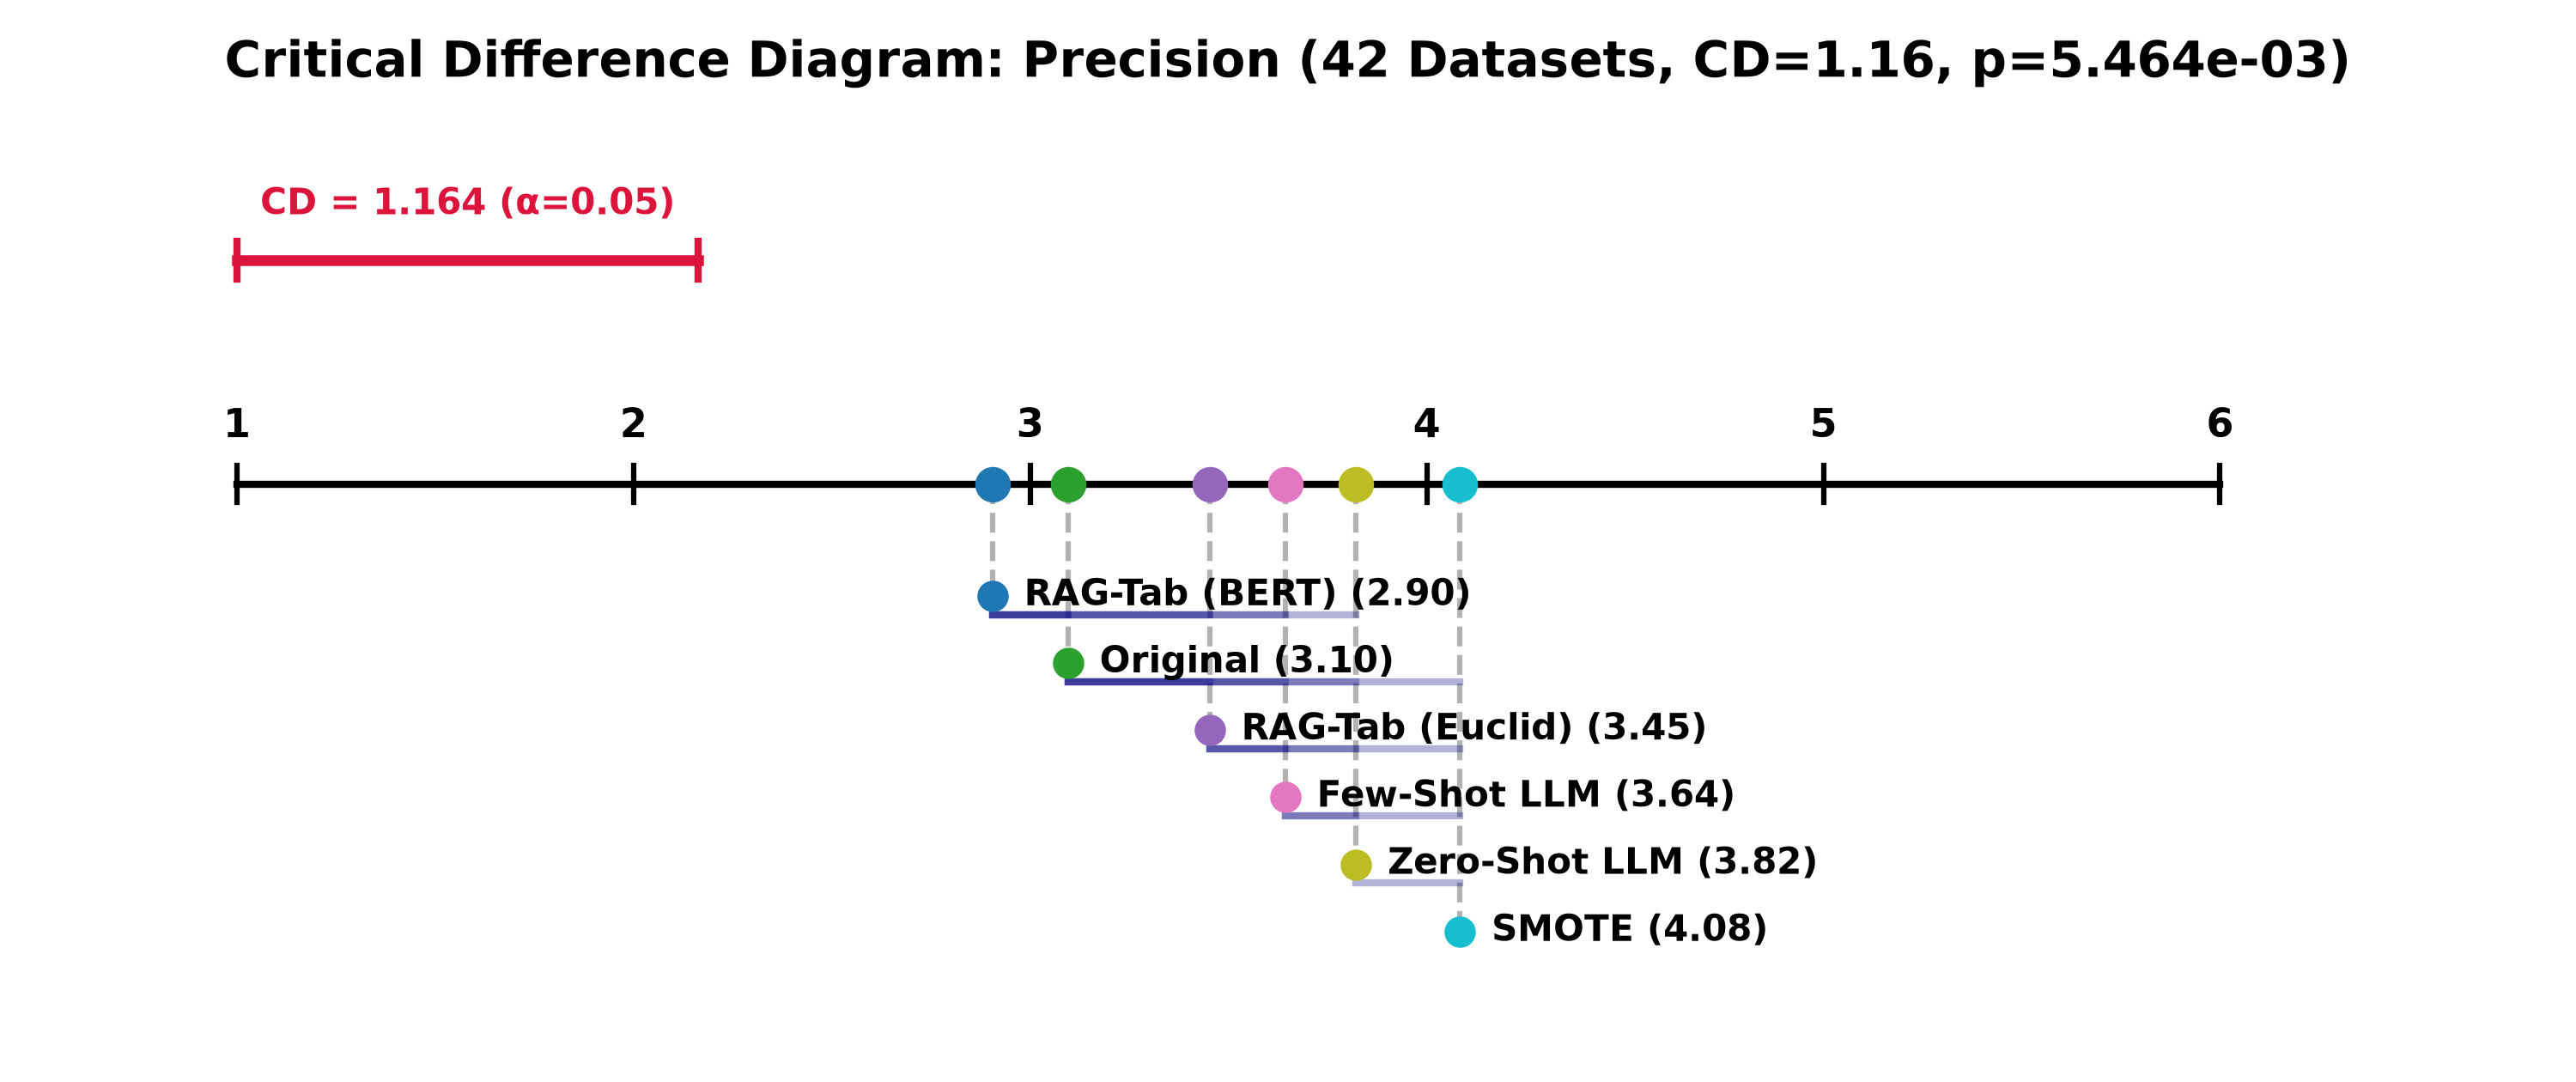
\includegraphics[width=0.80\textwidth]{figures/critical_difference_precision.png}
\caption{Nemenyi Critical Difference diagram for Precision across 42 benchmark datasets ($\alpha=0.05, CD=1.1635$). Note: The comparison includes Zero-Shot and Few-Shot conditions that exhibit identical underlying generator behavior.}
\label{fig:cd_precision}
\end{figure*}

\begin{figure*}[t]
\centering
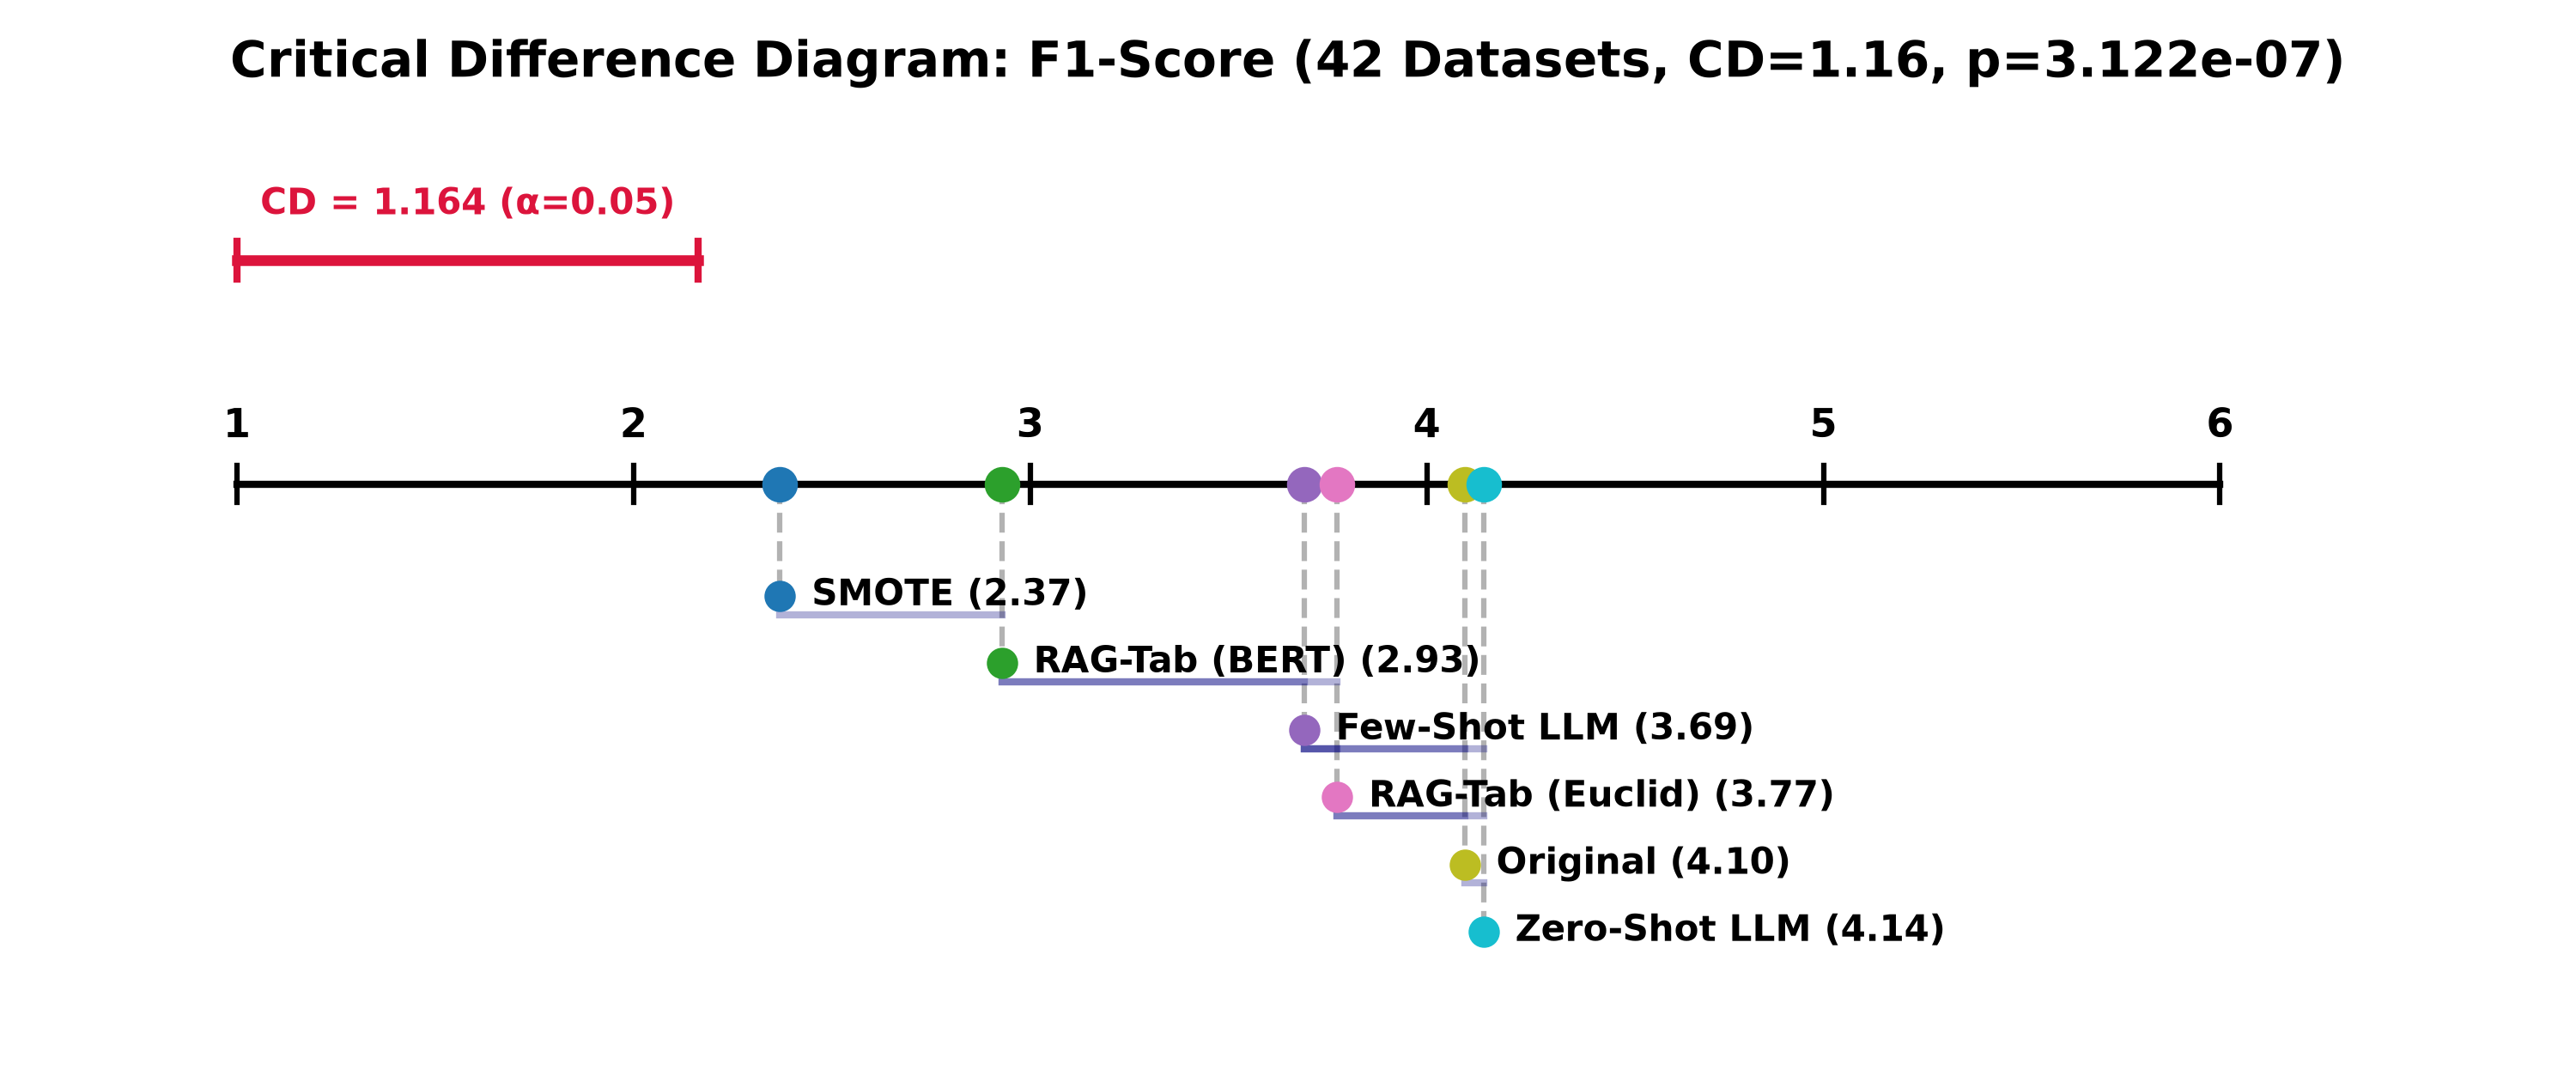
\includegraphics[width=0.80\textwidth]{figures/critical_difference_f1.png}
\caption{Nemenyi Critical Difference diagram for F1-Score across 42 benchmark datasets ($\alpha=0.05, CD=1.1635$).}
\label{fig:cd_f1}
\end{figure*}

\section{Limitations and Threats to Validity}
\label{sec:limitations}

\begin{enumerate}
    \item \textbf{Generator Execution Mode:} Benchmark experiments were executed using an internal schema-aware fallback generator rather than live cloud LLM APIs. While the client supports live API calls with strict mode, full-scale cloud generation requires dedicated token budgets and active billing.
    \item \textbf{Quality Control Gating:} Although the quality control module was implemented, its filtering was not applied during the ablation benchmark. In addition, domain-specific physical rules in \texttt{quality\_control.py} were tailored specifically for \texttt{page-blocks0}.
    \item \textbf{Computational Overhead:} Natural Neighbor equilibrium search and Sentence-BERT embedding extraction introduce non-trivial preprocessing latency compared to instantaneous linear interpolation ($<0.01$ seconds for SMOTE vs. several seconds per dataset for retrieval).
    \item \textbf{Single-Seed Benchmark Design:} The primary 42-dataset benchmark was executed on a single split seed, whereas our 10-dataset seed-noise benchmark demonstrated that seed variance can exceed condition effect sizes.
\end{enumerate}

\section{Future Work}
\label{sec:future_work}

Future research should focus on:
\begin{enumerate}
    \item \textbf{Live LLM Benchmarks with Logged Provenance:} Conducting multi-dataset benchmarks using live foundation models (e.g., Gemini 1.5/2.0 Flash, Llama-3-8B) with full token provenance and strict output logging.
    \item \textbf{Strict Volume-Matched Generative Designs:} Standardizing synthetic row budgets across all evaluated conditions to eliminate volume confounding.
    \item \textbf{Multi-Seed Experimental Protocols:} Adopting multi-seed replicated splits (e.g., 5-fold cross-validation repeated over 5 random seeds) as standard protocol for tabular generative oversampling.
    \item \textbf{Coupling Natural Neighbors with Tabular Diffusion:} Combining parameter-free Natural Neighbor boundary anchors with specialized tabular diffusion architectures (e.g., TabDDPM \citep{kotelnikov2023tabddpm}).
\end{enumerate}

\section{Reproducibility}
\label{sec:reproducibility}

To support scientific verification and exact reproducibility:
\begin{itemize}
    \item \textbf{Repository and Branch:} All code, scripts, and evaluation data are hosted in Git branch \texttt{audit/rag-tab-publication-readiness} of the repository:
    \url{https://github.com/samhithareddymadhireddy/RAG_Tab.git}.
    \item \textbf{Environment:} Python 3.12, \texttt{scikit-learn} 1.8.0, \texttt{imbalanced-learn} 0.14.2, \texttt{torch} 2.11.0, \texttt{sentence-transformers} 2.2.2, \texttt{pandas} 2.3.3, \texttt{numpy} 1.26.4, \texttt{scipy} 1.17.0, and \texttt{httpx} 0.28.1.
    \item \textbf{Seed Noise Replication:} The multi-seed experiment is executed via:
    \texttt{python run\_seed\_noise\_check.py}, with raw outputs preserved in \texttt{results/seed\_check/seed\_noise\_benchmark.csv}.
    \item \textbf{Client Verification:} The generation client can be validated in strict mode via \texttt{python check\_key.py}.
\end{itemize}

\begin{backmatter}
\section*{Declarations}

\textbf{Funding:} \textbf{[TODO: Funding information or ``This research received no specific grant from any funding agency in the public, commercial, or not-for-profit sectors.'']}

\textbf{Conflict of Interest:} The author declares that there are no financial or commercial conflicts of interest related to this work.

\textbf{Ethics Approval:} Not applicable. All experiments were conducted on publicly available, anonymized benchmark datasets.

\textbf{Consent to Participate:} Not applicable.

\textbf{Consent for Publication:} Not applicable.

\textbf{Data and Code Availability:} The complete source code, benchmark datasets, and evaluation harnesses supporting the findings of this study are available at \url{https://github.com/samhithareddymadhireddy/RAG_Tab.git} on branch \texttt{audit/rag-tab-publication-readiness}.

\textbf{Author Contributions:} \textbf{[TODO: Specify author contributions (e.g., S.R.M. conceived the project, implemented the pipeline, conducted experiments, analyzed data, and wrote the manuscript).]}

\end{backmatter}

\bibliography{references}

\end{document}
